\documentclass{beamer}
%\usepackage[spanish,activeacute]{babel}
\usetheme[sectionpage=none,progressbar=frametitle]{metropolis}
\usepackage[utf8]{inputenc}
\usepackage{listings}
\usepackage{amsmath,amsfonts,amssymb}
\usepackage{pmat}
\usepackage{color}
\usepackage{tikz}
\usetikzlibrary{positioning}
\usepackage{array}
%\usepackage{graphicx}
\usepackage{adjustbox}
\usepackage{booktabs}
\usetikzlibrary{shapes,arrows}
%\usepackage{multicol}
\usepackage{hhline}
\usepackage{pgf}
\usepackage{pgfplots}
\pgfplotsset{compat=1.12}
\usepackage{algorithm} 
\usepackage{algorithmic}
\renewcommand{\algorithmicrequire}{\textbf{Input:}}
\renewcommand{\algorithmicensure}{\textbf{Output:}}
\def\R{{\mathbb R }}
\def\N{{\mathbb N }}
\def\Z{{\mathbb Z }}

\makeatletter
%\setlength{\metropolis@titleseparator@linewidth}{2pt}
\setlength{\metropolis@progressonsectionpage@linewidth}{2pt}
\setlength{\metropolis@progressinheadfoot@linewidth}{2pt}
\makeatother


\definecolor{BlueTOL}{HTML}{222255}
\definecolor{BrownTOL}{HTML}{f43d00}%666633}
\definecolor{GreenTOL}{HTML}{225522}
\setbeamercolor{normal text}{fg=BlueTOL,bg=white}
\setbeamercolor{alerted text}{fg=BrownTOL}
\setbeamercolor{example text}{fg=GreenTOL}

\metroset{block=fill}

\setbeamercolor{block title alerted}{use=alerted text,
    fg=alerted text.fg,
    bg=alerted text.bg!80!alerted text.fg}
\setbeamercolor{block body alerted}{use={block title alerted, alerted text},
    fg=normal text.fg,
    bg=block title alerted.bg!50!alerted text.bg}
\setbeamercolor{block title example}{use=example text,
    fg=example text.fg,
    bg=example text.bg!80!example text.fg}
\setbeamercolor{block body example}{use={block title example, example text},
    fg=example text.fg,
    bg=block title example.bg!50!example text.bg}


\author[Paola Arce]{Paola Arce \\ Thesis advisor: Luis Salinas}
\date{December 15, 2017}
\title[Thesis defense]{Online learning methods for financial time series forecasting}
\subtitle{PhD Thesis Defense}
%
%\titlegraphic{
%    \tikz[overlay,remember picture]
%        \node[at=(current page.south east), anchor=south east] {
%            
\includegraphics[height=1.5cm]{img/DIT}
%        };
%}
%
%\author[Paola Arce]{Paola Arce}% \\ Thesis advisor: Luis Salinas}
%\date{December 11, 2017}
%\title[Thesis defense]{Fast and adaptive cointegration based model for forecasting financial time series}
%\subtitle{Seminario Inform\'atica CCTVal}



\begin{document}

\begin{frame}[plain]
\titlepage
\begin{tikzpicture}[overlay, remember picture]
\node[above right=0.4cm and 1.2cm of current page.south west] {
\includegraphics[width=2.5cm]{img/UTFSM}};
%\node[above =0.5cm of current page.south] {
\includegraphics[width=2cm]{img/DIT}};
\node[above left=0.5cm and .8cm of current page.south east] {
\includegraphics[width=5cm]{img/logo-di}};
\end{tikzpicture}

\end{frame}
%\usebackgroundtemplate{ } 

\begin{frame}
\frametitle{Outline}
\begin{itemize}
\item Motivation: High Frequency Trading and Cointegration
\item Challenges and Hypothesis
\item Contributions
\item Limitations and Applicability
\item Conclusions and Future Research
\end{itemize}
\end{frame}

\section{Motivation}


\begin{frame}
\frametitle{Motivation: HFT}
\begin{alertblock}{High Frequency Trading}
High Frequency Trading (HFT) is a technology that implements different trading strategies to buy or sell an stock using sophisticated infrastructure and high speed algorithms.
\end{alertblock}
HFT challenges are related to {\bf time series forecasting} and also {\bf computational} (hardware and software). Today, the volume of data has rapidly increased:
\begin{table}
\small
\begin{tabular}{ l | c }
Period & Data precision \\
\hline \hline
1993-2003 & seconds \\
2003-2015 & milliseconds \\
27th July 2015-onwards & microseconds \\
24th October 2016-onwards & nanoseconds
\end{tabular}
\caption{High Frequency data precision}
\end{table}
\end{frame}



\begin{frame}
\frametitle{HFT: High Frequency Trading}
High Frequency Trading has motivated computer-driven strategies capable of processing large amounts of data in short periods of time.
\begin{figure}
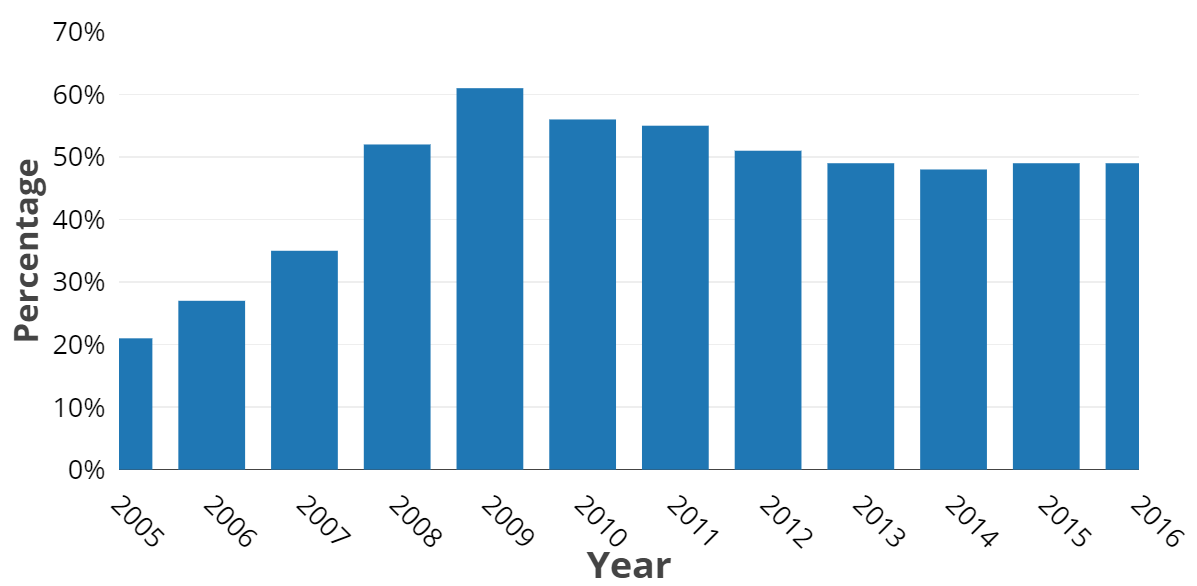
\includegraphics[width=0.7\paperwidth]{img/HFTmarket}
\caption{Percentage of HFT trades of total US Equity Trading. Source: TABB group}
\end{figure}
\end{frame}


\begin{frame}
\frametitle{HFT Revenue}
However, the revenues have fallen dramatically mainly because of more regulation, increasing the cost of HFT infrastructure and more competitive algorithms.
\begin{figure}
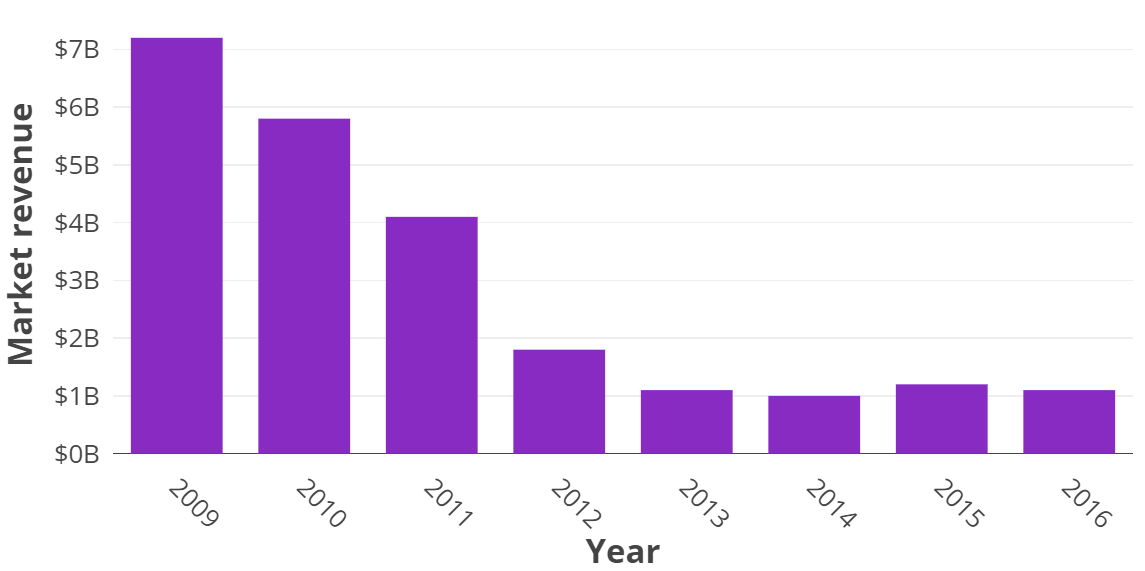
\includegraphics[width=0.7\paperwidth]{img/HFTmarket2}
\caption{Revenue in the US. Source: TABB group}
\end{figure}
\end{frame}

\begin{frame}
\frametitle{Motivation: HFT}
\begin{alertblock}{Arbitrage}
The practice of taking advantage of market inefficiency or discrepancies in the market price. Arbitrage contradicts the Efficient Market Hypothesis. 
%that states, the current stock price fully reflects available information related to its value and there is no way to earn excess profit.
\end{alertblock}
\begin{columns}

\begin{column}{0.5\textwidth}
\begin{exampleblock}{Advantages}
\begin{itemize}
\item Increases liquidity
\item Allows more efficient price formation
\item Reduce the difference between buyers (bid) and sellers (ask) prices.
\end{itemize}
\end{exampleblock}
\end{column}
\begin{column}{0.5\textwidth}
\begin{exampleblock}{Disadvantages}
\begin{itemize}
\item Removal of human decision making could lead to failures in untested or incorrect strategies
\item fairness
\end{itemize}
\end{exampleblock}
\end{column}
\end{columns}
\end{frame}


\begin{frame}
\frametitle{Motivation: Cointegration}
Cointegration reflects the idea of that some set of non-stationary variables cannot wander too far from each other.
\begin{figure}
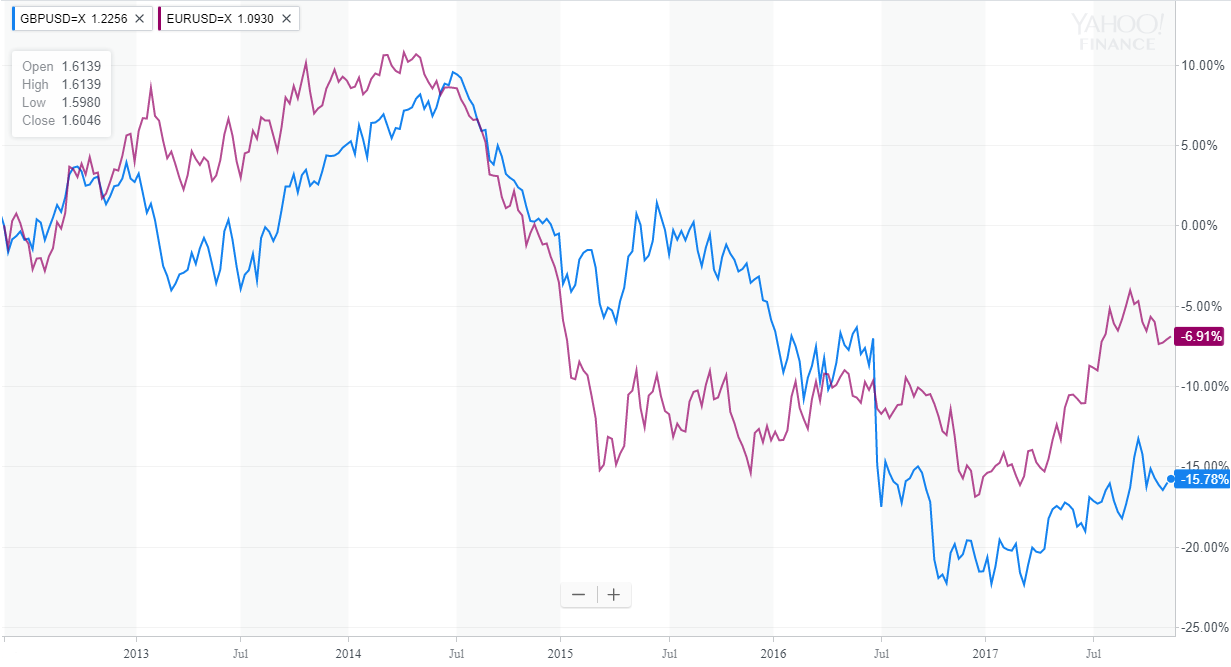
\includegraphics[width=0.8\paperwidth]{img/motivation}
\end{figure}
\end{frame}


\begin{frame}
\frametitle{Contribution}
This thesis contribution has several components:
\begin{figure}
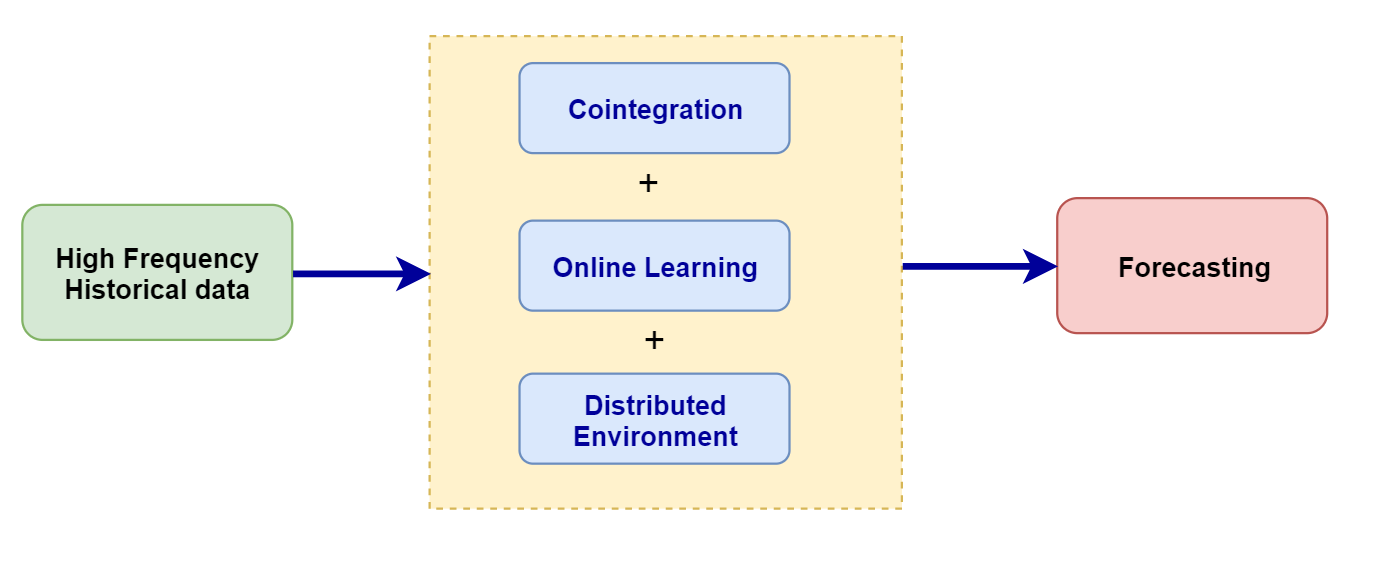
\includegraphics[width=\textwidth]{img/contribution}
\end{figure}
\end{frame}


\begin{frame}
\frametitle{High Frequency data}
High frequency time series are commonly:
\begin{columns}
\begin{column}{0.5\textwidth}
\begin{itemize}
\item Non-stationary
\item Irregularly spaced over time.
%\item Heterogeneity
\item Heteroscedastic
\item Potentially cointegrated
\end{itemize}
\end{column}
\begin{column}{0.5\textwidth}
\begin{figure}
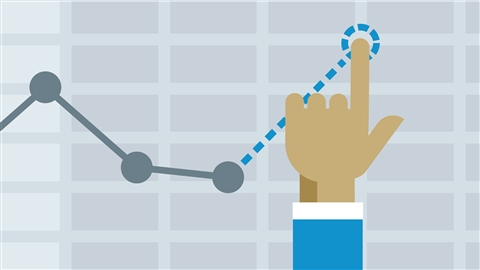
\includegraphics[width=0.35\paperwidth]{img/forecast}
\end{figure}
\end{column}
\end{columns}
\vspace{5mm}
This implies that classical statistical models as such can't be used. Therefore, financial time series forecasting is still a challenge.
\end{frame}

\begin{frame}
\frametitle{Stationarity}
\begin{block}{Strong definition}
A {\color{red}strictly stationary time series} $y_t: r.v$ with values in $\mathbb{R}$ defined for $t \in \mathbb{Z}$, is one for which the probabilistic behaviour of every collection of values $\{y_{t_1},y_{t_2},\dots,y_{t_L}\}$ is identical to that of the time shifted set, more precisely:
\begin{equation*}
{\color{blue}
P\{y_{t_1} \leq
c_1,..,y_{t_L} \leq c_L\} = P\{y_{t_1+h} \leq c_1,..,y_{t_L+h} \leq c_L\}\enspace }
\end{equation*}
\noindent $\forall L \in \mathbb{N}, \forall h \in \mathbb{Z}$, where $c_1,\dots,c_L$ are constants.
\end{block}
\end{frame}

\begin{frame}
\frametitle{Stationarity}
\begin{block}{Weak definition}

A weakly stationary time series is a process where the  mean, variance and auto covariance do not change over time:
\small
{\color{blue}
 \begin{eqnarray*} E(y_t) &=& \mu  \quad
\forall t \in \mathbb{N} \\ E(y^2_t) &=& \sigma^2  \quad \forall t \in
\mathbb{N} \\ \lambda(s,t)&=&\lambda(s+h,t+h) \quad \forall s,t \in \mathbb{N},
\forall h \in \mathbb{Z} \end{eqnarray*}}
\end{block}
\noindent with $\lambda(s,t) = E[(y_s-\mu)(y_t - \mu)]$ 
\end{frame}

\begin{frame}
\frametitle{Stationarity: consequences}
One of the consequences of stationary processes is how they recover from a shock. A shock represents an unexpected change in a variable in a particular period of time. For stationary time series, shocks to the system will gradually die away. 
\begin{figure}
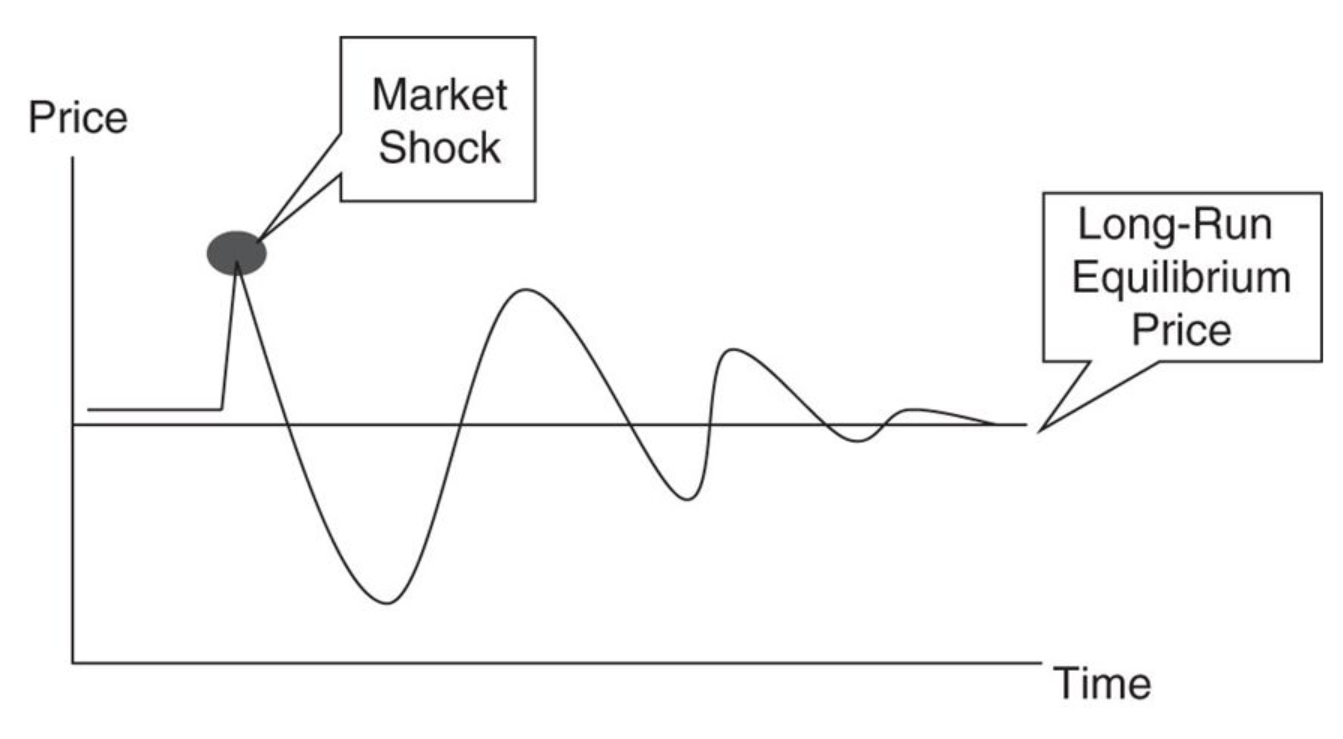
\includegraphics[width=0.6\paperwidth]{img/shock}
\end{figure}
\end{frame}


\begin{frame}
\frametitle{Non-stationary processes}
There are different types of non-stationary time series models often found in economics. Unit root process is one of them commonly used to model prices:
\begin{block}{Unit root process}
{\color{red}Unit root or I(1)} processes are also called stochastic trend if they have the following form:
{\color{blue}
\[
y_t = \mu + y_{t-1} + \epsilon_t
\]}
\noindent where $\epsilon_t$ is a stationary process. When $\mu = 0 $ the process is called {\bf pure random walk} and when $\mu \neq 0$  the process is called {\bf random walk with drift}.
\end{block}
\end{frame}


\begin{frame}
\frametitle{Integration }
\begin{block}{Integration of order $d$}
A time series $\mathbf{y}$ is said to be I(d), or integrated of order $d$, if after
differentiating the variable $d$ times, we get an stationary process, more precisely:
\[
{\color{blue}
(1-L)^d \mathbf{y} \sim \text{I(0)}} \, ,
\]
\noindent where I(0) is a stationary time series and $L$ is the lag operator:
\[
(1-L)\mathbf{y} = \Delta \mathbf{y}=\mathbf{y}_t  -\mathbf{y}_{t-1} \quad \forall t
\]
\end{block}
\end{frame}

\begin{frame}
\frametitle{Irregularly spaced over time}
\centerline{
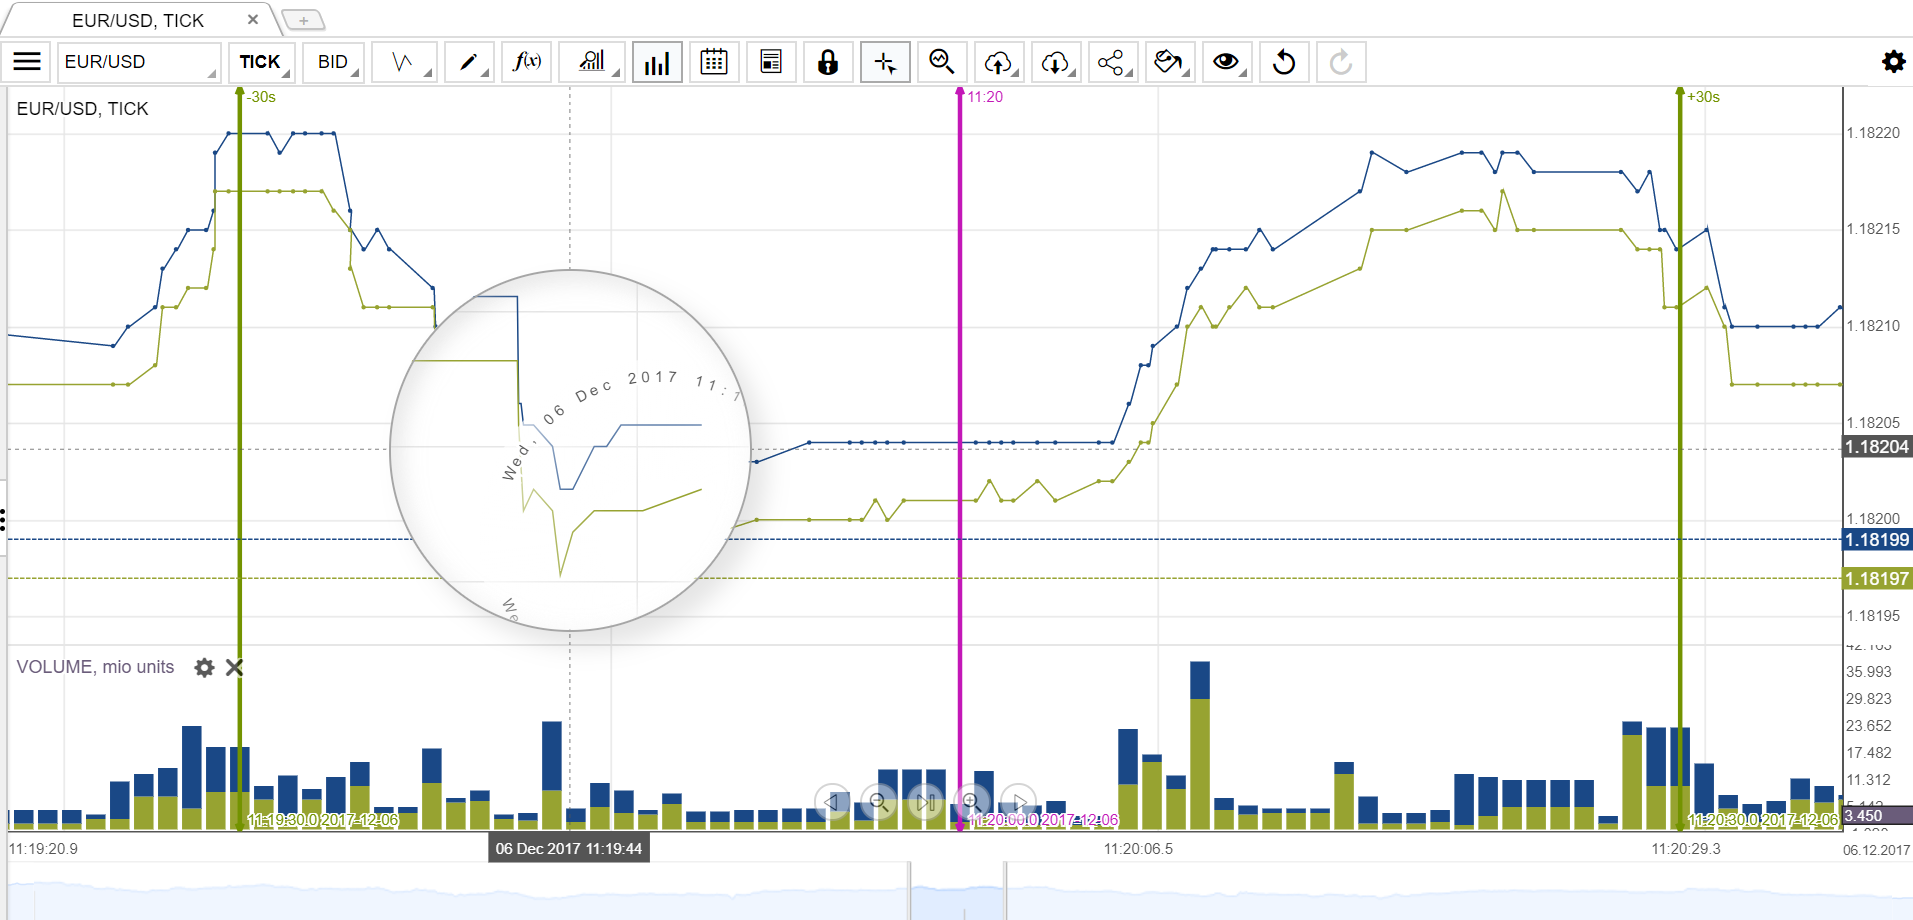
\includegraphics[width=\paperwidth,height=0.7\paperheight]{img/hft-ticks-zoom.png}
}
\end{frame}

\begin{frame}
\frametitle{Heteroscedastic}

\begin{block}{Heteroscedasticity}
Heteroscedasticity identifies {\bf non-constant volatility}.
Volatility gives a measure of uncertainty about future returns. It can either be obtained from historical returns or implied from derivatives such as options. 
\end{block}

\begin{figure}
\begin{tikzpicture}[ % Define Normal Probability Function
declare function={
            normal(\x,\m,\s) = 1/(2*\s*sqrt(pi))*exp(-(\x-\m)^2/(2*\s^2));
        }
       ]
\begin{axis}[
    no markers,
    domain=0:12,
    zmin=0, zmax=1,
    xmin=0, xmax=3,
    samples=200,
   samples y=0,
    axis lines=middle,
    xtick={0.5,1.5,2.5},
    xmajorgrids,
    xticklabels={},
    ytick=\empty,
    xticklabels={$\mathbf{y}_{t_1}$, $\mathbf{y}_{t_2}$, $\mathbf{y}_{t_3}$},
    ztick=\empty,
    xlabel=$t$, xlabel style={at={(rel axis cs:1,0,0)}, anchor=west},
    ylabel=$\mathbf{y}$, ylabel style={at={(rel axis cs:0,1,0)}, anchor=south west},
    zlabel=Probability density, zlabel style={at={(rel axis cs:0,0,0.5)}, rotate=90, anchor=south},
    set layers
  ]


\addplot3 [samples=2, samples y=0, domain=0:3] (x, {1.5*(x-0.5)+3}, 0);
\addplot3 [cyan!50!black, thick] (0.5, x, {normal(x, 3, 0.5)});
\addplot3 [cyan!50!black, thick] (1.5, x, {normal(x, 4.5, 1)});
\addplot3 [cyan!50!black, thick] (2.5, x, {normal(x, 6, 1.5)});

\pgfplotsextra{
\begin{pgfonlayer}{axis background}
\draw [on layer=axis background] (0.5, 3, 0) -- (0.5, 3, {normal(0,0,0.5)}) (0.5,0,0) -- (0.5,12,0);
\draw (1.5, 4.5, 0) -- (1.5, 4.5, {normal(0,0,1)}) (1.5,0,0) -- (1.5,12,0);
\draw (2.5, 6, 0) -- (2.5, 6, {normal(0,0,1.5)}) (2.5,0,0) -- (2.5,12,0);
\end{pgfonlayer}
}
\end{axis}


\end{tikzpicture}
\end{figure}
% An option is a contract which gives the owner the right but not the obligation to buy or sell an underlying asset at a given price called strike price.


\end{frame}

\section{Cointegration and the VECM model}


\begin{frame}
\frametitle{Cointegration definition}
%The idea of cointegration is that there is an I(1) process, underlying two or more processes.
\begin{block}{Cointegration}
The relationship between non-stationary time series can be modelled if a {\bf stationary linear combination} is shown to exist.
When this happens it is said they have a {\bf long-run
equilibrium} relationship and the variables are {\color{red} {\bf cointegrated}}.
\end{block}
\begin{figure}
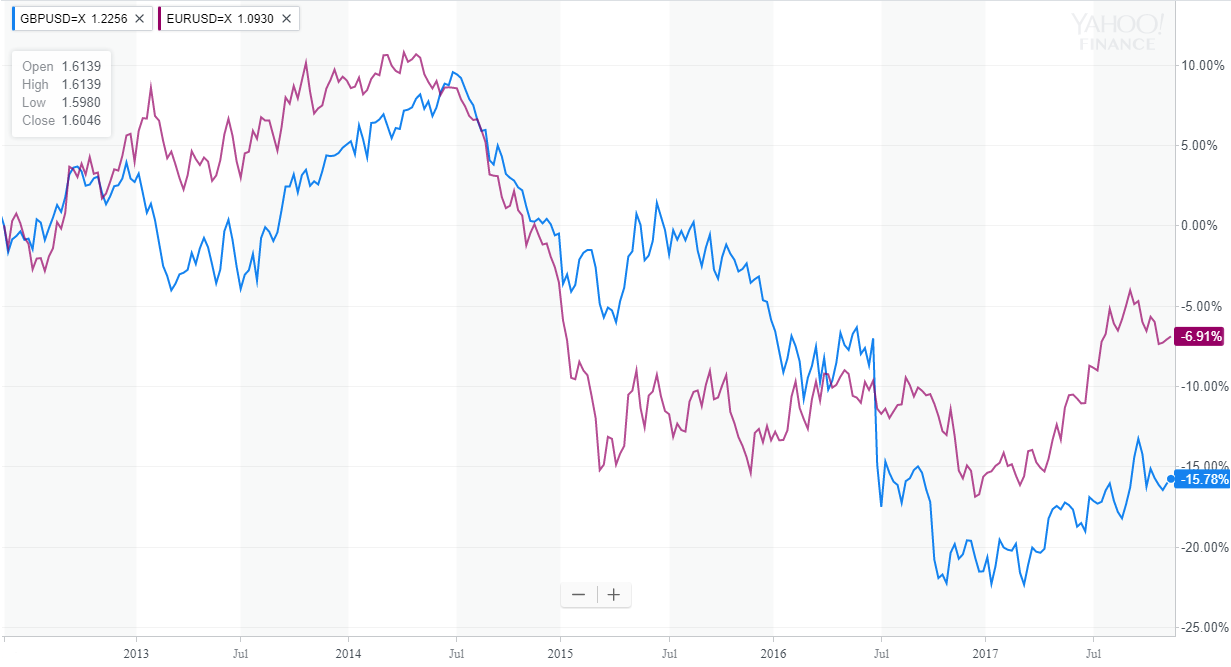
\includegraphics[width=0.8\paperwidth, height=0.4\paperheight]{img/motivation}
\end{figure}
\end{frame}

\begin{frame}
\frametitle{Cointegration: formal definition}
\begin{block}{Cointegration definition}
Let {\color{blue}$\mathbf{y} = \{\mathbf{y}^1, \dots, \mathbf{y}^l\}$} be a set of $l$
time series of order I(1) which are said to be cointegrated if a vector
${\color{blue}\boldsymbol\beta=[\beta(1),\dots,\beta(l)]^\intercal} \in \mathbb{R}^l$  exists such that the
time series,

\begin{equation*}
 \mathbf{Z}_t:= \boldsymbol \beta^\intercal \mathbf{y} = \beta(1) \mathbf{y}^1 + \dots + \beta(l) \mathbf{y}^l \sim
 \text{I(0)}\, .
\end{equation*}
\end{block}
%In other words, a set of I(1) variables is said to be cointegrated if
%a linear combination of them exists which is I(0).

\end{frame}


\tikzstyle{every picture}+=[remember picture]
\everymath{\displaystyle}
\begin{frame}
\frametitle{The Vector Error correction}
\tikzstyle{na} = [baseline=-.5ex]

The Vector Error correction model (VECM), considering $p$ lags, is used to model cointegrated time series:

{\Large
\begin{equation*}
 \Delta \mathbf{y}_t = \underbrace{
        \tikz[baseline]{
            \node[fill=red!20,ellipse,anchor=base] (t1)
            {$ \Omega\mathbf{y}_{t-1}$};
        }}_\text{Error correction term} +
        \underbrace{
        \tikz[baseline]{
            \node[fill=blue!20,anchor=base] (t2)
            {$\sum_{i=1}^{p-1} {\boldsymbol\phi}_i^* \Delta \mathbf{y}_{t-i} $};
        }}_\text{Autorregresive term} +
        \underbrace{
        \tikz[baseline]{
            \node[fill=green!20,anchor=base] (t3)
            {$c$};
        }}_\text{Intercept}
        +
        \underbrace{
        \tikz[baseline]{
            \node[fill=yellow!20,anchor=base] (t3)
            {$\boldsymbol{\epsilon}_t $};
        }}_\text{i.i.d}
\end{equation*}
}
\noindent where 
\begin{itemize}
\item $\mathbf{y}_t = [y^1_t,\dots,y^l_t]^\intercal$,
\item the errors $\mathbf{e}_t$ are assumed to follow i.i.d l-dimensional multivariate normal distribution $\mathcal{N}({\bf O,\Sigma})$, 
\end{itemize}
\end{frame}

\begin{frame}
\frametitle{The Vector Error correction}
\tikzstyle{na} = [baseline=-.5ex]

The Vector Error correction model (VECM), considering $p$ lags, is used to model cointegrated time series:

{\Large
\begin{equation*}
 \Delta \mathbf{y}_t = \underbrace{
        \tikz[baseline]{
            \node[fill=red!20,ellipse,anchor=base] (t1)
            {$ \Omega\mathbf{y}_{t-1}$};
        }}_\text{Error correction term} +
        \underbrace{
        \tikz[baseline]{
            \node[fill=blue!20,anchor=base] (t2)
            {$\sum_{i=1}^{p-1} {\boldsymbol\phi}_i^* \Delta \mathbf{y}_{t-i} $};
        }}_\text{Autorregresive term} +
        \underbrace{
        \tikz[baseline]{
            \node[fill=green!20,anchor=base] (t3)
            {$c$};
        }}_\text{Intercept}
        +
        \underbrace{
        \tikz[baseline]{
            \node[fill=yellow!20,anchor=base] (t3)
            {$\boldsymbol{\epsilon}_t $};
        }}_\text{i.i.d}
\end{equation*}
}
\noindent where 
\begin{itemize}
\item $\boldsymbol \Omega = \boldsymbol \alpha \boldsymbol \beta^\intercal$. The columns of $\boldsymbol\beta$ contains the cointegration vectors and the rows of $\boldsymbol\alpha$ correspond with the adjusted vectors.
\end{itemize}
\end{frame}




\begin{frame}
\frametitle{VECM limitations}

\begin{alertblock}{VECM limitations}
The Vector Error correction model is used to model cointegrated time series but only with {\bf batch data and rarely used with high frequency data} mainly due to {\bf computational limitations}:
\begin{itemize}
\item Calculation of the cointegration vectors $\boldsymbol \beta$ is obtained by the Johansen procedure which is of order $O(n^3)$.
%whereas $\alpha$ has to be determined as a variable in the VECM.
\item VECM parameters are obtained using the ordinary least squares ({\bf OLS}) method.
\end{itemize}
\end{alertblock}
\end{frame}

\begin{frame}
\frametitle{Online VECM}
Recently, online learning algorithms have been proposed to solve problems with large data sets mainly because of: 
\begin{itemize}
\item Their simplicity
\item They process one instance at a time
\item The hypothesis is updated every time new data arrives
\end{itemize} 
\end{frame}

\begin{frame}
\frametitle{Online learning algorithms}
\begin{algorithm}[H]
\begin{algorithmic}[1]
    \STATE Receives input $\mathbf{x}_t$
    \STATE Makes prediction $\mathbf{\hat{y}}_t$
    \STATE Receives response $\mathbf{y}_t$
    \STATE Incurs loss $l_t(\mathbf{y}_t,\mathbf{\hat{y}}_t)$
\end{algorithmic}
\caption{Structure of an Online Learning System}
\end{algorithm}
Performance is later measured after $T$ trials as:
\begin{equation*}
L_T = \sum_{t=1}^T l_t(\mathbf{y}_t,\mathbf{\hat{y}}_t)
\end{equation*}
\end{frame}


\section{Challenges and Hypothesis}
\begin{frame}
\frametitle{Challenge}
\begin{block}{Proposal}
To adapt VECM to be used with high frequency data, where the best parameters are updated when new data arrives.
\end{block}
\begin{exampleblock}{Hypothesis}
An algorithm based on cointegration and high performance computing will allow faster forecasting
algorithms for financial time series to be obtained while maintaining good accuracy levels.
\end{exampleblock}
\end{frame}

\section{Contributions}


\begin{frame}
\frametitle{Adaptive VECM}
\hspace*{-9mm}
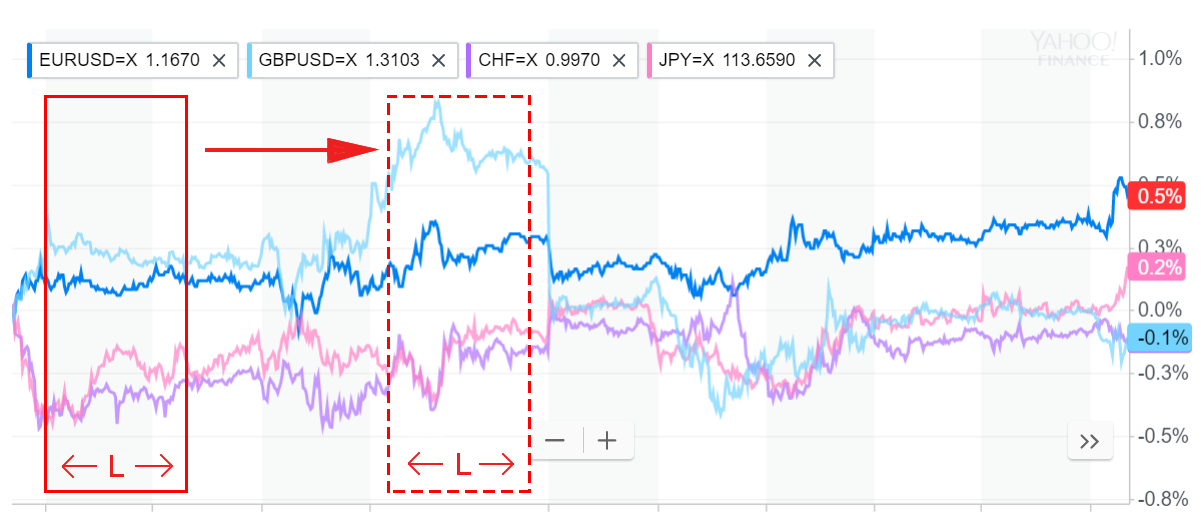
\includegraphics[width=1.15\textwidth]{img/slidingwindow}
\end{frame}


\begin{frame}
\frametitle{VECM(p) matrix form}
\begin{equation*}
 \Delta \mathbf{y}_t = \underbrace{
        \tikz[baseline]{
            \node[fill=red!20,ellipse,anchor=base] (t1)
            {$ \Omega\mathbf{y}_{t-1}$};
        }}_\text{Error correction term} +
        \underbrace{
        \tikz[baseline]{
            \node[fill=blue!20,anchor=base] (t2)
            {$\sum_{i=1}^{p-1} \phi_i^* \Delta \mathbf{y}_{t-i} $};
        }}_\text{Autorregresive term} +
        \underbrace{
        \tikz[baseline]{
            \node[fill=green!20,anchor=base] (t3)
            {$c$};
        }}_\text{Intercept}
        +
        \underbrace{
        \tikz[baseline]{
            \node[fill=yellow!20,anchor=base] (t3)
            {$\mathbf{\epsilon}_t $};
        }}_\text{i.i.d}
\end{equation*}
If we have $N$ data points, with $N>p$, the VECM matrix form is as follows:
\small
{\color{blue}
\begin{equation*}
\underbrace{
      \begin{bmatrix}
   \Delta\mathbf{y}_{p+1}^\intercal \\
   \Delta\mathbf{y}_{p+2}^\intercal \\
   \vdots \\
   \Delta\mathbf{y}_N^\intercal
   \end{bmatrix}}_{\mathbf{Y} } =
\arraycolsep=1.4pt
\underbrace{
\begin{pmat}[{....|}]
   \mathbf{y}_p^\intercal \boldsymbol{\beta} & \Delta \mathbf{y}_p^\intercal & \Delta\mathbf{y}_{p-1}^\intercal & \dots 
                    & \Delta\mathbf{y}_2^\intercal & 1 \cr
   \mathbf{y}_{p+1}^\intercal  \boldsymbol{\beta} &\Delta\mathbf{y}_{p+1}^\intercal & \Delta\mathbf{y}_p^\intercal & \dots
                       & \Delta\mathbf{y}_3^\intercal & 1 \cr
   \vdots & \vdots & \vdots & \ddots & \vdots & \vdots \cr
   \mathbf{y}_{N-1}^\intercal  \boldsymbol{\beta} &\Delta\mathbf{y}_{N-1}^\intercal & \Delta\mathbf{y}_{N-2}^\intercal & \dots 
                       & \Delta\mathbf{y}_{N-p-1}^\intercal & 1 \cr
   \end{pmat}}_{\mathbf{X}}
\underbrace{
   \begin{bmatrix}
   \boldsymbol{\alpha}^\intercal \\
   \boldsymbol{\Phi}_1^{*\top} \\
   \boldsymbol{\Phi}_2^{*\top} \\
   \vdots \\
   \boldsymbol{\Phi}_{p-1}^{*\top} \\
   \mathbf{c}^\intercal
   \end{bmatrix}
}_{\mathbf{W}}
+
\underbrace{
\begin{bmatrix}
   \boldsymbol{\epsilon}_{p+1}^\intercal \\
   \boldsymbol{\epsilon}_{p+2}^\intercal \\
   \vdots \\
   \boldsymbol{\epsilon}_N^\intercal \\
   \end{bmatrix}
}_{\mathbf{E}}
\end{equation*}}
%We can estimate the model parameters $\mathbf{W}$ using OLS:
%\begin{equation}
%{\color{blue}
%\mathbf{Y} = \mathbf{X}\mathbf{W}+\mathbf{E}
%}
%\end{equation}
\end{frame}

\begin{frame}
\frametitle{Online version of VECM}
VECM can be solved using a sliding windows of data, the problem can be expressed as follows:
 
{\color{blue}
\[
\mathbf{X}(t) = 
\begin{bmatrix} 
\mathbf{x}_{t-L}^\intercal \\ \vdots \\ \mathbf{x}_t^\intercal
\end{bmatrix} \; , 
{\bf Y}(t) = \begin{bmatrix} \mathbf{y}^\intercal_{t-L} \\ \vdots \\ \mathbf{y}^\intercal_t \end{bmatrix} \; .
\]
}

The optimal solution using a OLS is then:

{\color{blue}
\begin{eqnarray}
{\bf W}(t)_*&=&({\bf X}(t)^\intercal{\bf X}(t))^{-1}{\bf X}(t)^\intercal{\bf Y}(t) \\
&=&\Big( \displaystyle \sum_{i=0}^L \mathbf{x}_{t-i}
\mathbf{x}_{t-i}^\intercal \Big)^{-1} \displaystyle \sum_{i=0}^L \mathbf{x}_{t-i} \mathbf{y}^\intercal_{t-i}
\end{eqnarray}
}
\end{frame}


\begin{frame}
\begin{algorithm}[H]
\begin{algorithmic}[1]
\REQUIRE $\,$ \\
$\{\mathbf{x}_1,\dots,\mathbf{x}_N \}$: $N$ input vectors \\
$\{\mathbf{y}_1,\dots,\mathbf{y}_N \}$: $N$ targets \\
$L$: sliding window size ($L<N$) \\
\ENSURE  $\,$ \\
$\{f(\mathbf{x}_{L+1}),\dots,f(\mathbf{x}_N) \}$: model predictions \\
\STATE Initialize $\mathbf{A}=\displaystyle \sum_{t=1}^L \mathbf{x}_t
\mathbf{x}_t^\intercal$
and $\mathbf{b}=\displaystyle \sum_{t=1}^L \mathbf{x}_t \mathbf{y}^\intercal_{t}$
\FOR { $t = L+1$ to $N$ }
        \STATE read new $\mathbf{x}_t$
        \STATE $\mathbf{A} = \mathbf{A} + \mathbf{x}_t \mathbf{x}_t^\intercal-
\mathbf{x}_{t-L-1} \mathbf{x}_{t-L-1}^\intercal  $
        \STATE output prediction $f(\mathbf{x}_t) =  \mathbf{b}^\intercal
\mathbf{A}^{-1}\mathbf{x}_t$
        \STATE Read new $\mathbf{y}_t$
        \STATE $\mathbf{b} = \mathbf{b} + \mathbf{x}_t \mathbf{y}^\intercal_{t}$
\ENDFOR
\end{algorithmic}
\caption{Online Ordinary Least Squares}
\label{alg:SLAAR}
\end{algorithm}
\end{frame}

\begin{frame}
\frametitle{How to choose $L$?: $\boldsymbol \Omega$ matrix properties}
Since $\boldsymbol \Omega = \boldsymbol \alpha \boldsymbol \beta^\intercal$ we can also say that:
$$\boldsymbol \Omega \mathbf{y} = \boldsymbol \alpha \boldsymbol \beta^\intercal \mathbf{y} = \boldsymbol \alpha \mathbf{Z}_t \sim \text{I(0)}$$
The matrix $\boldsymbol \Omega$ has the following properties:
\begin{itemize}
\item If ${\color{blue}rank(\boldsymbol \Omega) = 0}$ there is no cointegration
\item If ${\color{blue}rank(\boldsymbol\Omega)=l}$ i.e full rank, $\boldsymbol\Omega$ is non-singular or invertible, therefore we can express $\mathbf{y}$ as follows:
$$\mathbf{y} = \boldsymbol \Omega ^{-1} \boldsymbol \alpha \mathbf{Z}_t \sim \text{I(0)} \, ,$$
then the time series are not I(1) but stationary.
\item If ${\color{blue}rank(\boldsymbol\Omega)=r,\quad 0 < r < l}$ then, r cointegration vectors exist such that: 
$$\boldsymbol \Omega \mathbf{y} = \boldsymbol \alpha \mathbf{Z}_t \sim \text{I(0)} \, .$$
%where $\boldsymbol\alpha$ and $\boldsymbol\beta$ are $(l \times r)$
%matrices and $rank(\boldsymbol\alpha)=rank(\boldsymbol\beta)=r$.
\end{itemize}
\end{frame}


\begin{frame}
\frametitle{How to choose L?}
  \begin{figure}[!h]
  %\vspace{-0.8cm}
  \centering
   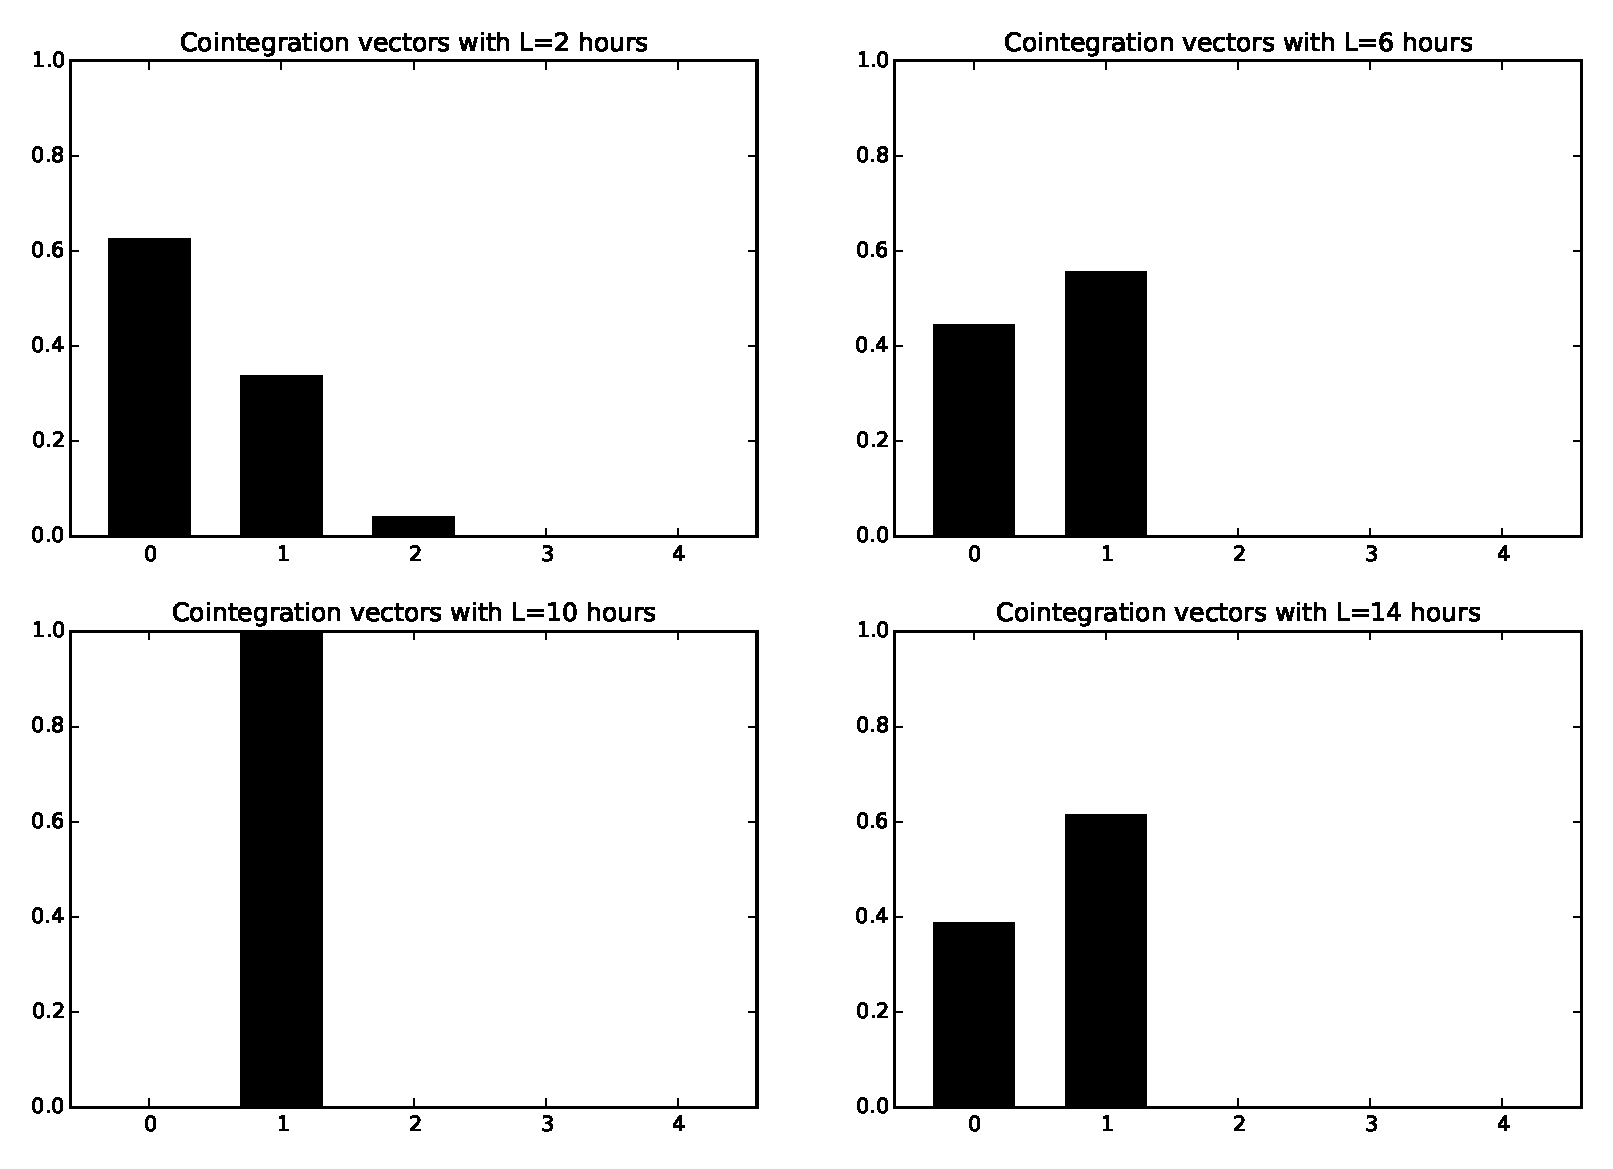
\includegraphics[width=0.85\textwidth]{img/51_Fig1}
  \caption[Distribution of the number of cointegration vectors using $p=1$ lags]{Distribution of the number of cointegration vectors using $p=1$ lags.}
  %Four possible values for windows size $L$ are shown (2, 6, 10 and 14) hours (1 hour = 360 data points).}
  \label{fig:hists}
\end{figure}
\end{frame}


\begin{frame}
\frametitle{Percentage of cointegration}
Since $r=0$ means no cointegration and $r=l=4$ reveals that no process is I(1) but stationary.
The interesting cases of cointegration are those where $r$ lies strictly
between $0$ and $l$, i.e. $0<r<l$.
\vspace{5mm}
\begin{block}{Percentage of cointegration (PC)}
{\color{blue}
\begin{equation*} \label{eq:pcoint}
PC = 
\frac{\#\{ it \mid \text{$it$ has $r$ c.v. with $0<r<l$}\}}
     {\#it}\times 100
\end{equation*}}
\end{block}
\end{frame}

\begin{frame}
\frametitle{Data}
\begin{columns}
\begin{column}{0.7\textwidth}
\begin{itemize}
\item This data was collected from {\bf Dukascopy}, a free
database which gives access to the {\bf Swiss Foreign Exchange marketplace}.
\item Tests were carried out using four foreign exchange rates all related to
USD: {\bf EURUSD, GBPUSD, USDCHF} and {\bf USDJPY}. 
\item The tests were done using {\bf 10-seconds frequency} from ask prices
from the 11th to the 15th of August 2014. 
%\item Since one day corresponds to 8640 data points and we used 5 days of data, we have 43,200 data points in total.
\end{itemize}
\end{column}
\begin{column}{0.3\textwidth}
 \begin{figure}[!h]
    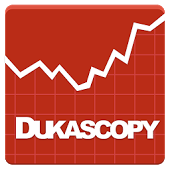
\includegraphics[width=\textwidth]{img/dukascopy}
 \end{figure}
\end{column}
\end{columns}
\end{frame}


\begin{frame}
\frametitle{PC vs MSE}
\begin{figure}[ht!]
  %\vspace{-0.8cm}
  \centering
  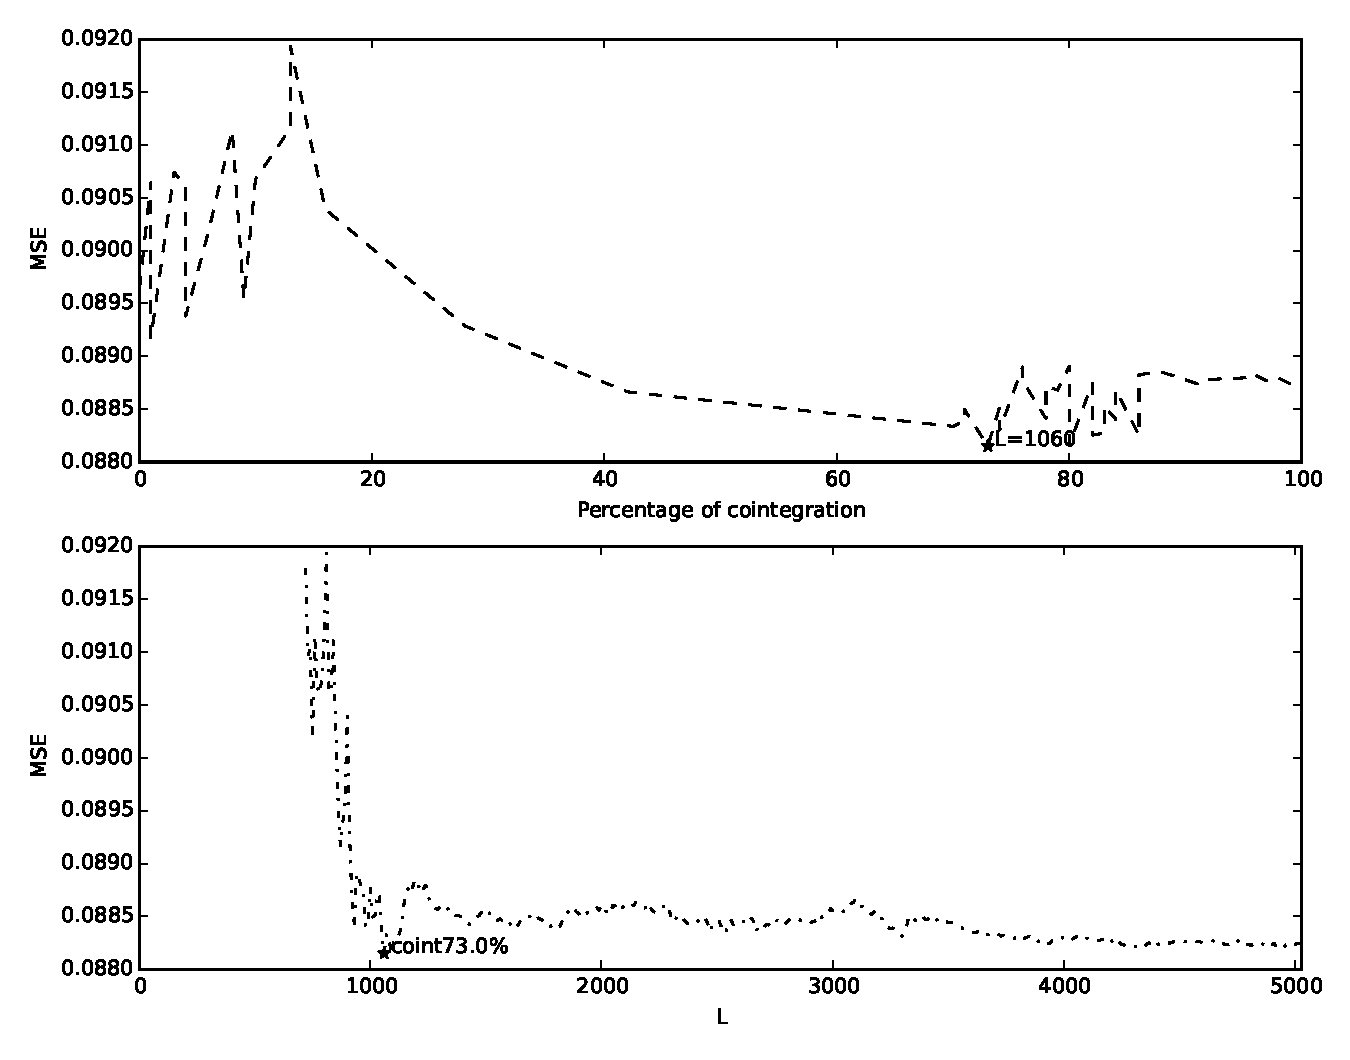
\includegraphics[width=0.8\textwidth]{img/51_Fig2}
  \caption{MSE versus the percentage of cointegration considering 1000
  iterations. }
  \label{fig:cointvsmse}
\end{figure}
\end{frame}

\begin{frame}
\frametitle{Adaptive VECM algorithm (AVECM)}
\begin{enumerate}
\item It uses VECM only considering a sliding windows of size $L$ of data.
\item We proposed to choose $L$ and the number of lags $p$ in order to maximise the percentage of cointegration $PC$ in the near past. This process was done every time that new data was processed. 
\item And to use a distributed environment to make this parameters search, since this is the most expensive routine.
\end{enumerate}
\end{frame}






%%\begin{frame}
%%\frametitle{Evaluation methods}
%%\begin{block}{MSE}
%%Measures the distance between forecasts
%%and the true values and large deviations from the true value have a
%%large impact due to squaring forecast error.
%%{\color{blue}
%%\begin{equation}\label{eq:MSE}
%%\text{MSE} = 
%%\frac{\displaystyle \sum_{t=1}^{N} (\mathbf{y}_t-\hat{\mathbf{y}}_t)^2}{N}
%%\end{equation}}
%%\end{block}
%%\begin{block}{\bf $U$-statistic}
%%Unit free measure obtained as the ratio between the root MSE (RMSE) of a model and the RMSE of the naive random walk model. 
%%\end{block}
%%\end{frame}
%
%\section{Experiments}
%\subsection{Uno}
%
\begin{frame}
\frametitle{Unit root tests}
Augmented Dickey Fuller (ADF) test with lags $p=1,2,3,4,5$.
\begin{table}[ht]
\centering
\small
\begin{tabular}{llllll}
\toprule
{Variable} & {ADF(1)} & {ADF(2)} & {ADF(3)} & {ADF(4)} & {ADF(5)}\\ 
\midrule
EURUSD &  -0.052   & -0.054  & -0.054  & -0.054  & -0.054  \\
GBPUSD &  -0.744  & -0.784  & -0.805  & -0.837  & -0.846  \\
USDCHF &  -0.476   & -0.493  & -0.493  & -0.495  & -0.502  \\
USDJPY &  0.357   & 0.360  & 0.360  & 0.367  & 0.367  \\
$\Delta$ EURUSD & -128.4*  & -128.4*  & -96.85* & -89.12*   & -89.12*\\
$\Delta$ GBPUSD & -131.4*  & -112.7*  & -102.5* & -92.86*   & -88.29*\\
$\Delta$ USDCHF & -127.8*  & -127.8*  & -96.94* & -88.82*   & -80.79*\\
$\Delta$ USDJPY & -135.1*  & -135.1*  & -101.2* & -101.2*   & -101.2*\\
\bottomrule
\addlinespace[1ex]
\end{tabular}
\caption{Unit roots tests for EURUSD, GBPUSD, USDCHF and USDJPY at 10-second
frequency.}
\label{tab:adf}
\end{table}
\end{frame}

\begin{frame}
\frametitle{Performance accuracy}
\small
\begin{tabular}{ccccccc}
& \multicolumn{3}{l}{{\bf MSE}} & &
\multicolumn{2}{c}{{\bf $\mathbf{U}$-statistic}} \\ 
\hhline{~---~--} \\
 & AVECM & ARIMA & p-value & &
AVECM & ARIMA \\ 

\hline
 EURUSD & 1.0702 e-09 & 1.1481 e-09 &  \bf{9.250 e-12} & & {\color{GreenTOL}\bf{0.6863}} & {\color{red}\bf{0.7108}}\\
 GBPUSD & 1.6630 e-09 & 1.7408 e-09 &  6.951 e-02 & & {\color{GreenTOL}\bf{0.6866}} & {\color{red}\bf{0.7025}}\\
 USDCHF & 5.8503 e-10 & 6.3545 e-10 &  \bf{2.899 e-14} & & {\color{GreenTOL}\bf{0.6803}} & {\color{red}\bf{0.7091}}\\
 USDJPY  & 6.3483 e-06 & 6.5194 e-06 &  \bf{6.853 e-05} & & {\color{GreenTOL}\bf{0.6964}} & {\color{red}\bf{0.7057}}
 \end{tabular}
 \end{frame}
%%For AVECM we considered different number of iterations (parameter $m$ in algorithm \ref{alg:AVECM}): 10, 50 and 100. We tried 12, 24 and 47 different pair of combinations for $L$ and $p$. Possible values for $L$ were in the interval $[100,4000]$ and $p$ can have values in between $[1,5]$. Best AVECM performance was compared against ARIMA and the random walk model.
%%Table~\ref{tab:stats} shows the out-of-sample performance measures: MSE and $U$-statistic for AVECM and ARIMA. In terms of both measures we found that AVECM is superior to ARIMA and the naive random walk model. We also included the p-value that proves that the difference in the MSE is significant at the 99\% significance level in three of the four currency rates and at 90\% in the case of GBPUSD. The $U$-statistic shows that AVECM and ARIMA are superior to the naive random walk model and that our proposal is also superior to ARIMA.
%
%
%
\begin{frame}
\frametitle{Parallel implementation}
The function that get optimal parameters $L$ and $p$ was implemented using MPI in Python. Tests ran in our cluster {\bf hpc.utfsm.cl} considering 2 servers Xeon E5-2667 (2.90GHz) of 24 cores each (48 cores in total) and 24GB RAM.

Parameter settings:
\begin{itemize}
%\item Parameter $it=100$
\item The $L$ parameter was always chosen between 100 and 4000 (1 hour=360 data points) and $p$ always took values between 1 and 5. 
\item Parameter $nparams$ represents the number of pairs ($L$,$p$) used to maximise the percentage of cointegration. 
\end{itemize}
\end{frame}
%
\begin{frame}
\frametitle{Execution times}
\begin{figure}[ht]
  \centering
  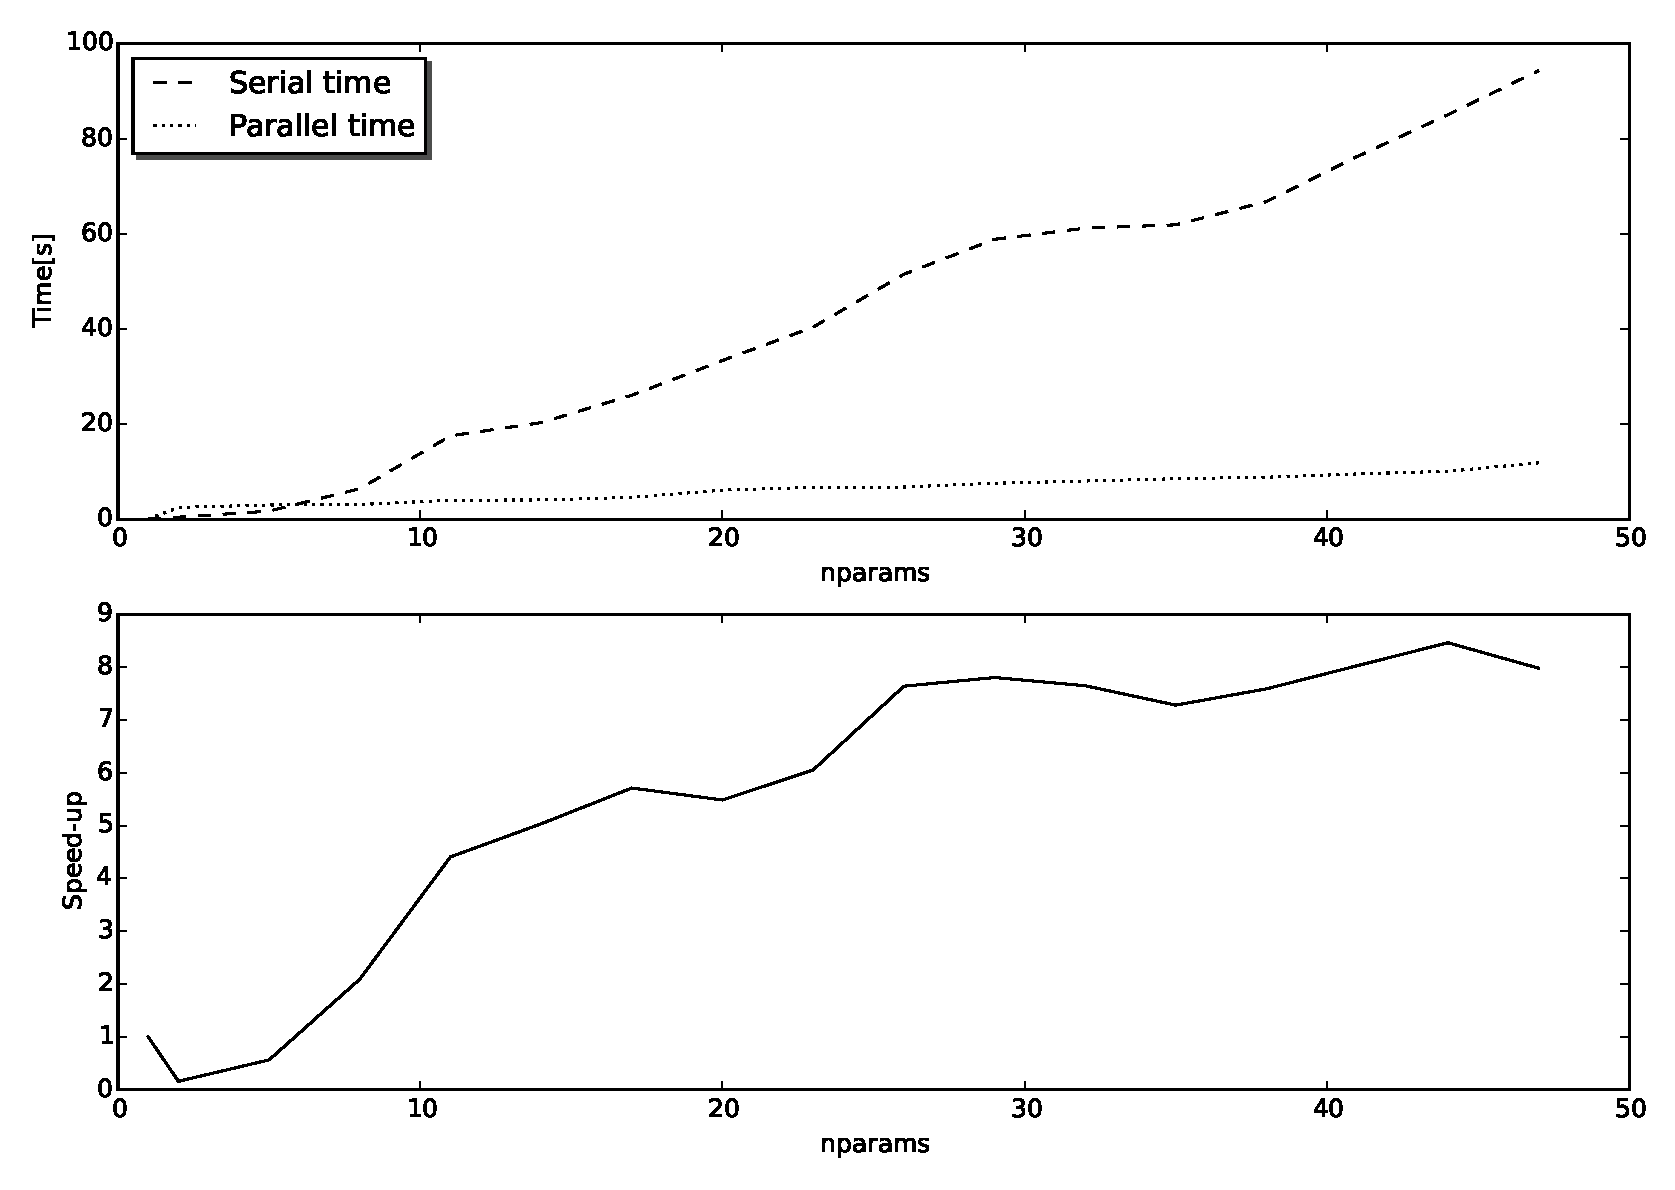
\includegraphics[width=0.9\textwidth]{img/51_Fig3}
  \caption[Computing time and Speed-up]{Computing time of sequential and parallel algorithm is shown in the
  upper figure. Speed-up is shown below.}
  \label{fig:extimes}
\end{figure}
\end{frame}

\begin{frame}
\frametitle{Contributions}
%\begin{figure}
%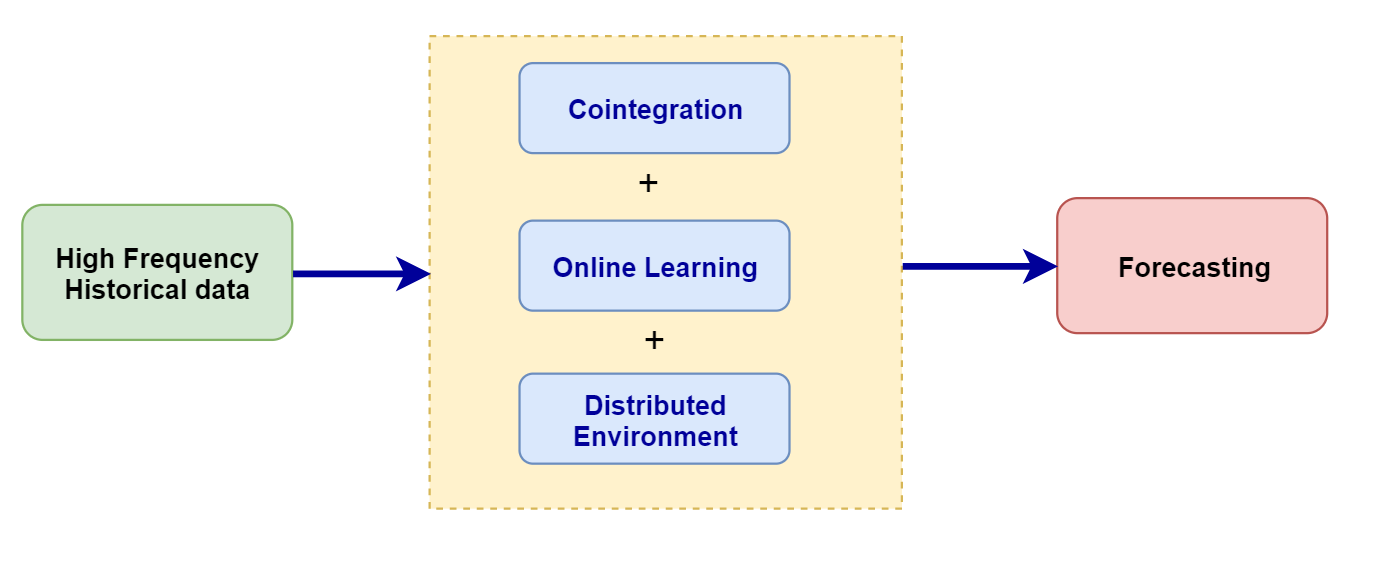
\includegraphics[width=0.7\textwidth]{img/contribution}
%\end{figure}
\begin{description}
\item[Cointegration]Cointegration relations change with time. We empirically showed that the number of coitegration vectors is sensitive to the number of lags but also to the amount of data considered. The percentage of cointegration is used to find VECM parameters.
\item[Online learning] The adaptation of the VECM to be used in an online context expressing the OLS method with matrix actualization.
\item[Distributed environment] The use of a distributed environment to calculate $L$ and $p$ and obtain a response below 10 seconds.
\end{description}
\end{frame}

\section{Limitations and Applicability}

\begin{frame}
\frametitle{Limitations and Applicability}
\begin{itemize}
\item Cointegration information can be used as an integration tool to detect arbitrage opportunities.
\item Use with stocks, forex rates and crypto-currency?
\item Applicable to other non-stationary but cointegrated time series
\end{itemize}
\end{frame}

\section{Conclusions and Future Research}

\begin{frame}
\frametitle{Conclusions}
\begin{itemize}
%\item We found that out-of-sample forecast performance MSE is related to the {\em percentage of cointegration\/}.  
\item AVECM improves performance measures by finding parameters of $L$ and $p$ maximising the percentage of cointegration.
\item AVECM performance is superior to ARIMA and the naive random walk model in terms of MSE and $U$-statistic. 
%This result is very important since it is still difficult to outperform ARIMA and the random walk model for standard econometric forecasting models  despite their simplicity.
\item We showed that VECM computational limitations can be tackled using a an online approach in a distributed environment.
\end{itemize}
\end{frame}


\begin{frame}
\frametitle{Articles and conferences}
\nocite{arce+salinas2012,icpram15,Arce2017}
\bibliographystyle{apalike}
\bibliography{reference}
\end{frame}


\begin{frame}
\frametitle{Future research}
\begin{itemize}
\item To add {\bf matrix optimizations} to obtain VECM parameters.
\item To add a regularization parameter to get better generalisation capabilities using {\bf Ridge Regression} and the {\bf Aggregating Algorithm for Regression}.
\item To include {\bf more explicative variables} such as bid-ask spread and change in volume.
\item The online approach for {\bf other econometrics models} it is also worthy of  study.% Many of them could be adapted and used with higher frequency data.
\end{itemize}
\end{frame}



\begin{frame}[plain,c]
\begin{center}
\Huge Thank you for your attention
\Huge Questions?
\end{center}
\end{frame}



%\begin{frame}
%\hspace*{-4mm}
%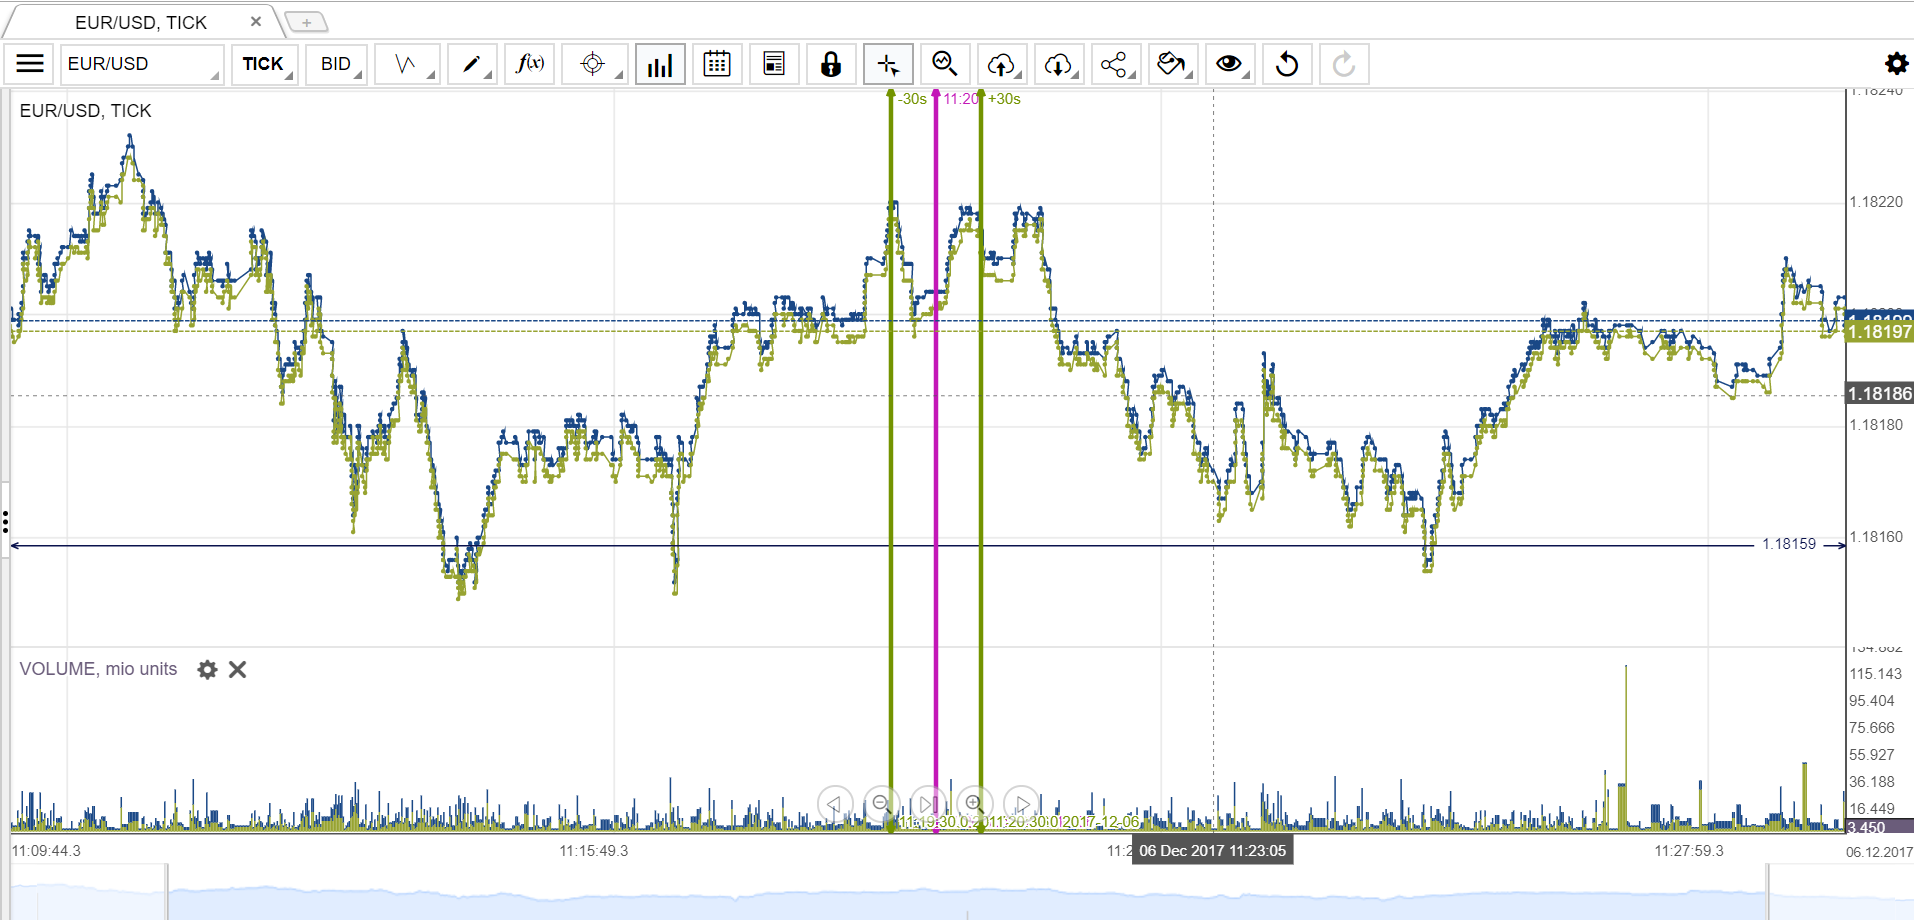
\includegraphics[width=\paperwidth]{img/hft-ticks.png}
%\end{frame}
%



%Have a slide for each of the following
%9 Problem statement or Hypothesis
%9 “Why is this a Hard Problem?”
%9 Approach or Methodology
%9 “Why is this Innovative?”
%9 Assumptions and Constraints
%9 Initial Results (Promise of Great Things to Come)
%9 Validation Plan

%9 Expected Contributions
%9 “What’s beyond this thesis?”
%9 Roadmap of Thesis

\appendix

\begin{frame}
\frametitle{Stationarity}
A time series $y_t: \Z \to \R $ is said to be strictly stationary if, for a finite set of $L$ indices $\{t_{1},\dots,t_{L}\}  \, \forall L \in \Z_{\ge 0}$, the joint probability distribution of the random variables $\{y_{t_{1}},y_{t_{2}},\dots,y_{t_{L}}\}$ remains unchanged for any time shifted $h$.
The probability distribution for the random variable $y_{t_1}$ is:

\begin{equation}
P\{y_{t} \leq c_1 \} = P\{t \in \Z:  y_t \in  ]-\infty, c_1] \} 
\end{equation}


\end{frame}

\begin{frame}
\frametitle{The order book}
\begin{figure}
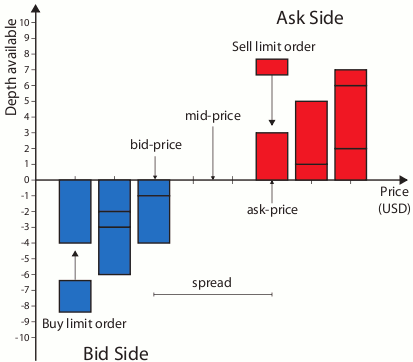
\includegraphics[width=0.7\textwidth]{img/orderbook}
\end{figure}
\end{frame}

\begin{frame}
\frametitle{Unit root process}

\end{frame}


\begin{frame}
\frametitle{Integration example}
\begin{columns}
\column[t]{5cm}
High frequency financial time series are commonly an I(1) process 
\begin{center}
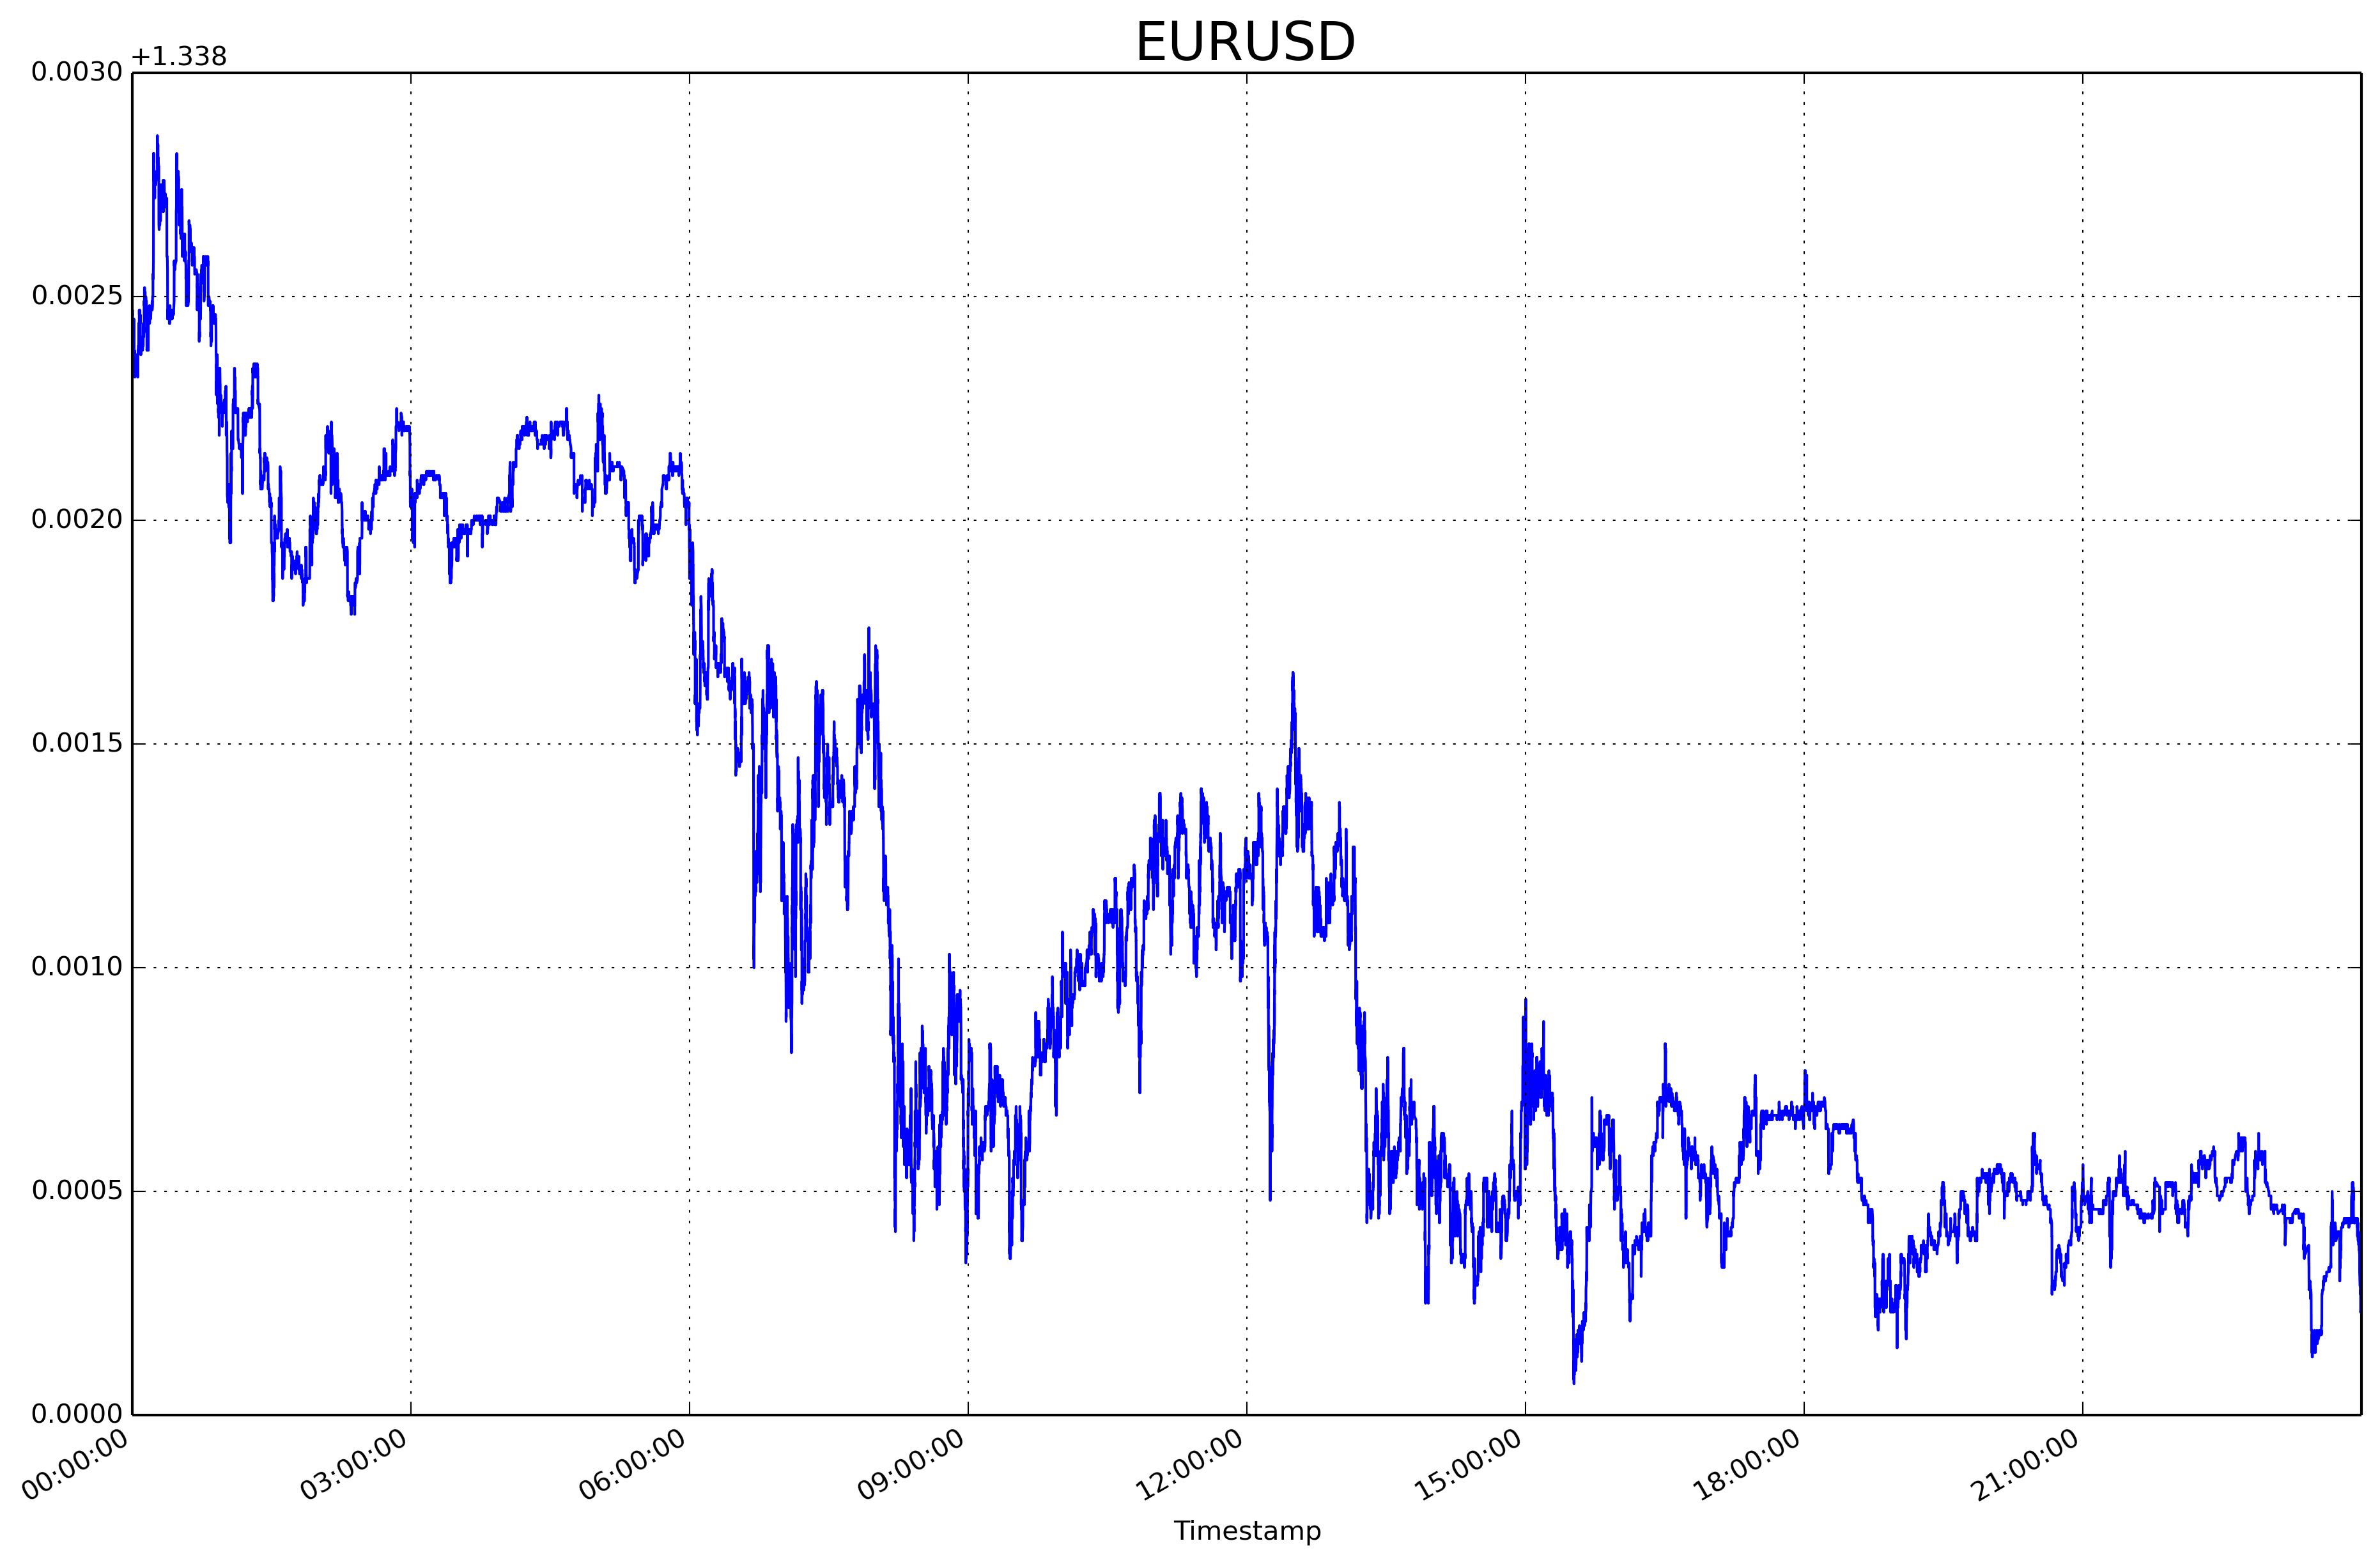
\includegraphics[width=0.85\textwidth]{img/EURUSD}
\end{center}
\column[t]{5cm}
Since their differences are stationary (I(0) process).
\newline
\begin{center}
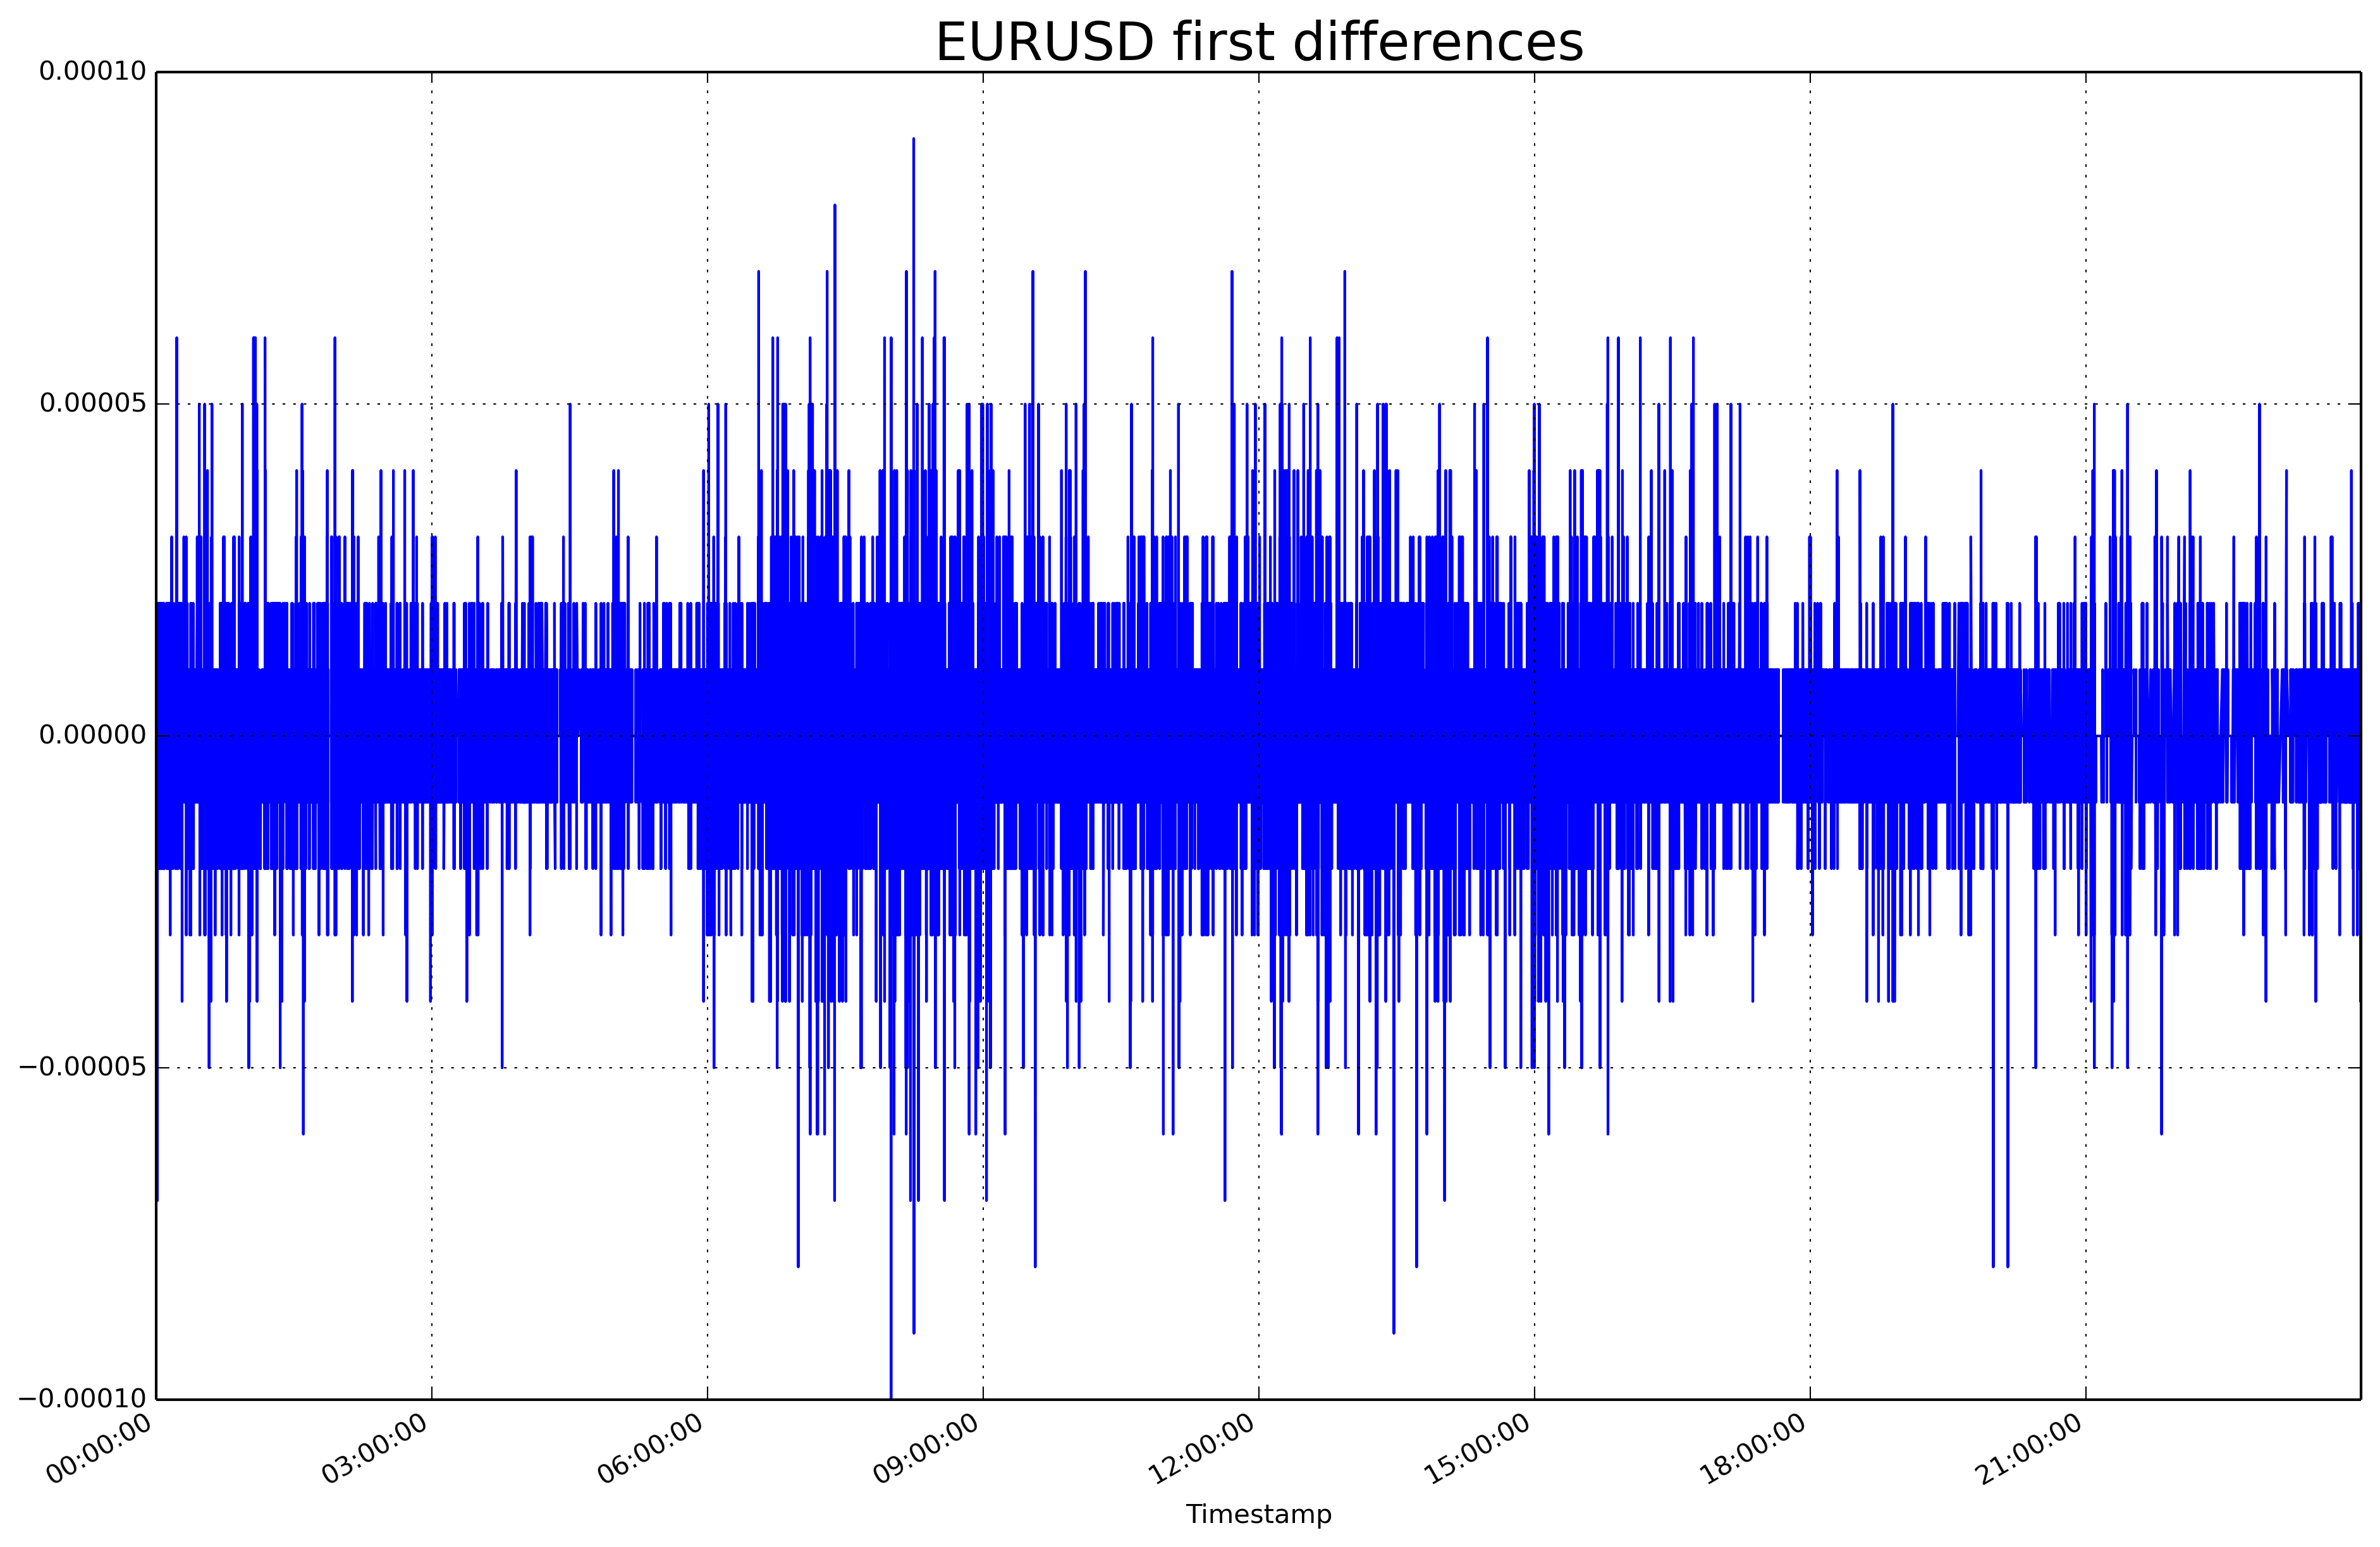
\includegraphics[width=0.85\textwidth]{img/DEURUSD}
\end{center}
\end{columns}
\end{frame}

\begin{frame}
\frametitle{Spurious regression}
Standard regression techniques are applied to non-stationary data.
The use of non-stationary data can lead to spurious regressions.  

%\begin{block}{Spurious regression}
%If two stationary
%variables are generated as independent random series and are trending over time, when one of those variables is regressed on the other, they could have a high coefficient of determination ($R^2$) even if the two are totally unrelated. 
%\end{block}

\begin{columns}
\begin{column}{.45\linewidth}<1->
\begin{figure}
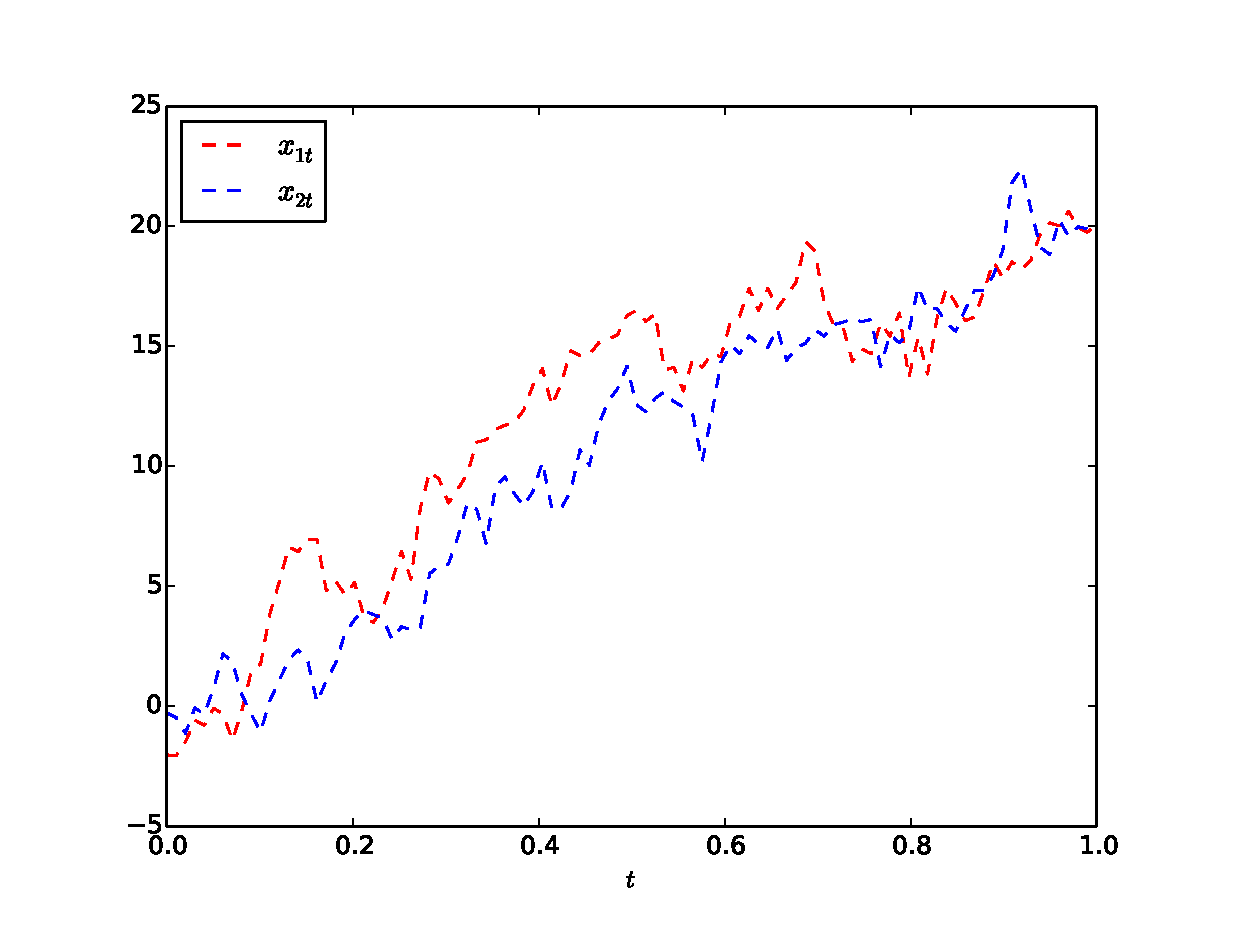
\includegraphics[width=0.4\paperwidth]{img/spurious1}
\end{figure}
\end{column}
\begin{column}{.45\linewidth}<2->
\begin{figure}
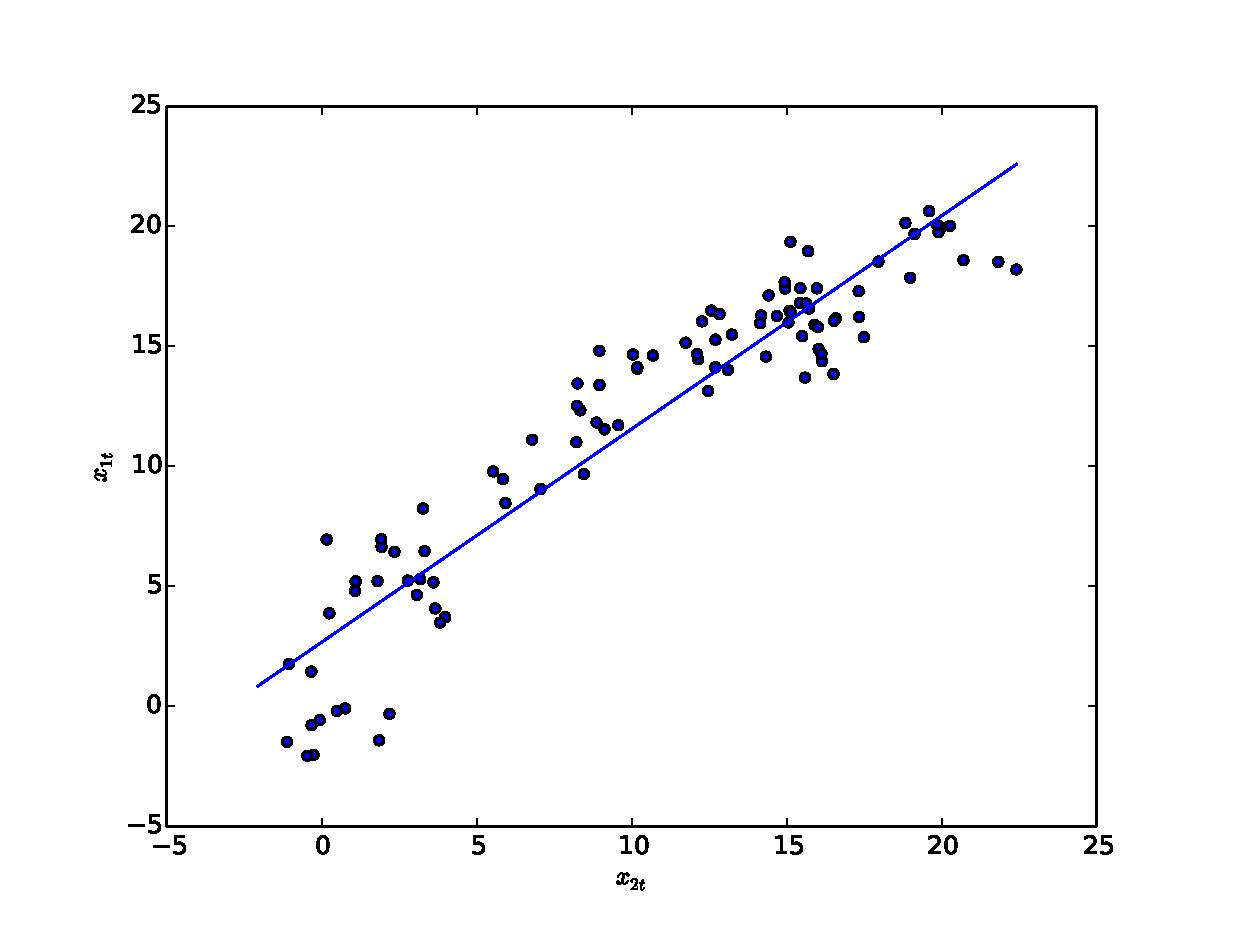
\includegraphics[width=0.4\paperwidth]{img/spurious2}
\end{figure}
\end{column}
\end{columns}
\end{frame}

\begin{frame}
\frametitle{Random walk}
The random walk model is defined as:
\begin{equation}
\mathbf{y}_t = \mathbf{y}_{t-1} + \epsilon_{t}
\label{rwmodel}
\end{equation}
The naive forecast of the time series difference $\hat{\mathbf{y}}_{t+1}$ for the random walk model is defined as:
\begin{equation}
\hat{\mathbf{y}}_{t+1} = \mathbf{y}_t + \hat{\epsilon}_{t+1} 
\end{equation}
\noindent where  $\hat{\epsilon}_{t+1} = \epsilon_{t}$.
\end{frame}
%
%
\begin{frame}
\frametitle{ARIMA}
A process can be modelled as an ARIMA$(p,d,q)$ if $\mathbf{x}_t = \Delta^d \mathbf{y}_t $, is an ARMA$(p,q)$. An ARMA$(p,q)$ model is the following:
\begin{equation}
\mathbf{x}_t = \sum_{i=1}^p \phi_i \mathbf{x}_{t-i}  +  \sum_{j=1}^q \theta_j \epsilon_{t-j}  
\end{equation}
\noindent with coefficients $\phi_p \neq 0$, $\theta_q \neq 0$ and $\sigma_{\epsilon}^2 > 0$.
\end{frame}



\begin{frame}
\frametitle{AVECM Algorithm}
\small
\begin{algorithmic}[1]
\REQUIRE $\,$ \\
$\mathbf{y}$: matrix with $N$ input vectors and $l$ time series\\
$j$: Starting point of testing \\
$it$: Ending point of testing \\
$ps$: list of $p$ values \\
$Ls$: list of $L$ values ($L<N$) \\
$m$: Iterations to determine parameters ($m < N-L$)\\
\ENSURE  $\,$ \\
$\{ \hat{\mathbf{y}}[1],\dots,\hat{\mathbf{y}}[it]\}$: prediction vectors \\
\FOR { $i =j$ to $it$ }
   \STATE $\mathbf{Y} \gets \mathbf{y}[:,i-1]$
    \STATE $L,p \gets
    \texttt{get\_best\_params}(Ls,ps,m,\mathbf{Y})$
        \STATE $model = \text{VECM}(\mathbf{Y},L, p)$
        \STATE $\hat{\mathbf{y}}[i-j] = model.predict()$
\ENDFOR
\end{algorithmic}
\end{frame}

% Financial time series are not the only ones with this behaviour, this study can be extended to other non-stationary time series such as: weather, earthquakes, energy demand and sales forecasting.


\end{document}
